\cotefile{62}
\scanpage{2}

Courbes elliptiques

\mspage{1}

\scanpage{4}

\uline{Modules des courbes elliptiques}

Soit $C$ une ``courbe elliptique'' homogène sur $S$ loc. noethérien. La section nulle $s$ définit un bon diviseur $D$ sur $C$ \inserted{transversal aux fibres}, d'où un \deleted{fibré}, \inserted{faisceau inv. $\underline L$} dont les \inserted{germes de} sections sont des \deleted{fonctions} germes de fonctions sur $C$ (précisément celles qui sont des ``multiples'' de $D$). Noter que \deleted{$s^*(\underline L)\simeq$}, $C$ étant un schéma en groupes
\[
\unsure{\underline T_{C/S}|\underline{\mathcal T}_{C/S}}=f^*(s^*(\underline T_{C/S}))=f^*(\mathcal L_{C/S})
\]
\margin{[$\mathcal L$ : faisceau de Lie]}

\deleted{\uline{Proposition 1} les $L^n$ $(n\in\mathbb Z)$ sont \unsure{cohomolgt|cohomologt} plats en \unsure{ttes|toute} dimension.}
\[
s^*(\underline L)\simeq s^*(\underline L\underset C\otimes\underline O_{S'})\simeq s^*(\underline N_{C/S'})\simeq s^*(\underline T_{C/S})\simeq\unsure{\mathcal L}
\]
Ce faisceau sera noté $\mathcal L_{C/S}$ [``Lie'']. Donc
\[
s^*(\underline L^{\otimes n})\simeq\mathcal L_{C/S}^{\otimes n}
\]

On a une section \unsure{évidente} de $\underline L$, savoir la section constante $1$ de $\underline O_C$,
\[
\sigma:\underline O_C\longrightarrow\underline L\qquad \sigma\in\Gamma(C,\underline L)
\]
qui définit un homomorphisme (\unsure{d'injections linéaires})
\diagram{\begin{tikzcd}[column sep=small]
\cdots\arrow[r]&\underline L^{\otimes n}\arrow[r,dash]&\underline L^{\otimes(n+1)}\arrow[r]&\cdots\arrow[r]&\underline L^{\otimes(n+\unsure{h})}\arrow[r]&\cdots
\end{tikzcd}}
\margin{$\subset$ faisc. des fonctions rationnelles \unsure{relatives} sur $C/S$}
\unsure{d'où} \deleted{\unsure{un}} des homomorphismes
\diagram{\begin{tikzcd}[column sep=large]
\cdots\arrow[r]&f_*(\underline L^{\otimes n})\arrow[r]&f_*(\underline L^{\otimes(n+1)})\arrow[r]&\cdots
\end{tikzcd}}
i.e.
\diagram{\begin{tikzcd}
\cdots\arrow[r]&\mathcal E_n\arrow[r,dash]&\mathcal E_{n+1}\arrow[r]&\cdots
\end{tikzcd}}
en posant $\mathcal E_n=f_*(\underline L^{\otimes n})$

\mspage{3}

\scanpage{5}

\uline{Proposition 1} Les faisceaux $\underline L^{\otimes n}$ sont coh. plats en \unsure{tte} dimension. Le faisceau $f_*(\underline L^{\otimes n})$ est localement libre, de rang $0$ si $n<0$, $1$ si $n=0$ ou $1$, $n\deleted{\unsure{+1}}$ si $n\geq1$. \deleted{\unsure{Le}} Le faisceau $\underline L$ est ample, et de façon précise $\underline L^{\otimes n}$ est \deleted{\unsure{très}} \uline{ample} \deleted{pour} \inserted{ssi} $n\geq1$, très ample ssi $n\unsure{\geq|>}3$.

La formule de RR, où $g=1$, d'où $2g-2=0$, nous montre que \uline{tout faisceau} \deleted{loc. libre} inversible sur $C$, de degré \inserted{relatif} $d\neq0$, est coh. plat, et que sa dimension est \deleted{\unsure{donc}} nulle si $d<0$, et $d\deleted{\unsure{-(g-1)}}$ si $d\geq1$. Donc la première assertion est démontrée pour $n\neq0$, et pour $n=0$ elle est connue par ailleurs, car $\underline L^{\otimes0}=\underline O_C$.
\margin{prop. préliminaire sur un faisceau inversible \unsure{quelconque}}
\inserted{On sait aussi qu'un faisceau inv. sur $C$ de degré relatif $d$ est ample ssi $d>0$, donc $\underline L^{\otimes n}$ est ample ssi $n\geq1$. \deleted{\unsure{Et puisque}}}
\deleted{Comme $\underline L$ est de degré relatif $1>0$, il est ample, \unsure{par suite} \unsure{les} $\underline L^{\otimes n}$ est très ample pour $n\unsure{\gg|>}0$.}

Si $\underline L^{\otimes n}$ est très ample, on a $n\geq1$, d'ailleurs on ne peut avoir $n=1,2$ car alors $\unsure{\mathbb P|P}(f_*(\underline L^{\otimes n}))$ est de dim relative $0$ ou $1$, donc $C$ ne peut s'y immerger (car il y serait isomorphe, absurde), donc il faut $n\geq3$.

\unsure{Ceci suffit}, car à cause de la platitude cohomologique, on est ramené au cas où $S=\operatorname{Spec}k$, $k$ un corps \inserted{alg. clos}. \deleted{Mais alors D'ailleurs, comme $\underline L$ est engendré loc. par ses sections}

Mais \deleted{alors} comme $3>(2g-2)+2=\uline{2g}=2$, un raisonnement connu n'utilisant que RR donne le résultat.

\mspage{4}

\scanpage{6}

\uuline{Proposition} On a donc des \deleted{\unsure{hom}} inclusions
\[
\mathcal E_0=\mathcal E_1\subset\mathcal E_2\subset\mathcal E_3\subset\cdots
\]
les $\mathcal E_i$ sont des faisceaux loc. libres de rang $i$ pour $i\geq1$. D'ailleurs
\[
\mathcal E_0=\underline O_S
\]

\uline{Proposition 2} $\mathcal E_0=\mathcal E_1=\underline O_S$, d'autre part pour $i\leq j$ l'injection $\mathcal E_i\longrightarrow\mathcal E_j$ est \deleted{\unsure{locale}} universellement injective.
\deleted{Le faisceau} \inserted{Soit} $\mathcal L_n\simeq\mathcal E_{\unsure{n}}/\mathcal E_{n-1}$ \inserted{(pour $n\geq\unsure{0|2}$, \deleted{\unsure{$\mathcal L_0=\underline O_S$}}) \unsure{les $\mathcal L_i$, soit $i\neq1$}; alors on a des isomorphismes} \deleted{est isomorphe à $\mathcal L^{\otimes\unsure{k}}$, et $\mathcal E_{n+1}/\mathcal E_n$ est isomorphe à $\mathcal L^{\otimes n}$.}
\[
\mathcal L_n\otimes\mathcal L_m\simeq\mathcal L_{m+n}\qquad\text{si }n,m\begin{cases}\geq0\\\neq1\end{cases}
\]
\inserted{provenant de} \deleted{\unsure{faisant de}} \inserted{une structure} sur $\coprod_{n\geq0}\mathcal L_n$ \deleted{\unsure{une}} d'Algèbre graduée comm.

Pour la première assertion, \unsure{avec|grâce à} la platitude coh. on est ramené au cas d'un corps, où c'est trivial car on a une injection.

Notons que $\mathcal E=\varinjlim\mathcal E_n=f_*(\varinjlim\underline L^{\otimes n})$ est une $\underline O_S$-\uline{Algèbre}, dont la connaissance d'ailleurs implique la connaissance de $\underline\Gamma_*^{\unsure{\mathcal E}}(f,\underline L)=\coprod\mathcal E_n$, car $\mathcal E_m\times\mathcal E_n\unsure{\longrightarrow|-}\mathcal E_{m+n}$ est précisément induit par la multiplication de $\mathcal E$. On a, en passant au \unsure{gr. ann.} associé à la filtration croissante donnée, une Algèbre $\coprod_{n\geq0}\underline{\mathcal L}_n$, où les $\underline{\mathcal L}_n\simeq\mathcal E_n/\mathcal E_{n-1}$ pour $n\geq0$, en modifiant pour $n=0$ par $\underline O_S$. Il faut prouver que
\[
\underline{\mathcal L}_n\otimes\underline{\mathcal L}_m\unsure{\longrightarrow|-}\underline{\mathcal L}_{n+m},\qquad n,m\begin{cases}>0\\\neq1\end{cases},\quad\deleted{n,m}
\]
est bien isom., ou encore surjectif, \deleted{\unsure{et pour}} Si $n$ ou $m=0$, \deleted{\unsure{ramenons nous} \illegible{3} \unsure{au voisinage}} c'est trivial, sinon on a $n,m\geq2$, et on voit.

\mspage{5}

\scanpage{7}

on est ramené à ceci.

\uline{Corollaire} Si $n\geq2$, $\underline{\mathcal L}_n$ est isomorphe par les hom \unsure{induits} à $\underline{\mathcal L}_2^{\otimes n'}$ si $n$ pair, à $\underline{\mathcal L}_2^{\otimes n'}\otimes\underline{\mathcal L}_3$ si $n$ impair (où $n'\geq1$ dans le premier cas, $n'\geq0$ dans le deuxième).

Mais on a plutôt intérêt de procéder directement ainsi : On est ramené aussitôt par platitude coh. au cas où $S=\operatorname{Spec}k$, on prend alors un élément $f$ de $L_n$ non dans $L_{n-1}$, un $g$ de $L_m$ non dans $L_{m-1}$, donc $fg$ est dans $\unsure{L_{n+m}|L_{n+m}^{0}}$ mais \unsure{provient} par \unsure{déf. de} $L_n\otimes L_m$.

\uline{Corollaire} $\mathcal E_3$ engendre $\Gamma_*(f,\underline L)$

Considérons les opérations de $\underline T$ sur les germes de fonctions rationnelles sur $C$ [reste à définir], on constate que \deleted{\unsure{$\underline T$}} ces opérations induisent des hom
\[
\underline{\mathcal L}\otimes\underline{\mathcal L}_n\longrightarrow\underline{\mathcal L}_{n+1}\qquad n\geq2
\]

\uline{Proposition 3} \inserted{Soit $s\in S$, $p$ l'exp. car. de $k(s)$.} L'homomorphisme $\underline{\mathcal L}\otimes\underline{\mathcal L}_n\unsure{\longrightarrow|-}\underline{\mathcal L}_{n+1}$ est un \uline{isomorphisme} (ou \deleted{\unsure{est}} un \unsure{épim.}) ssi $p$ est premier à $n$.

On est ramené au cas où $S=\operatorname{Spec}k$, alors c'est une vérification locale : si $D$ est une \deleted{\unsure{diff}} dérivation inv. non nulle en un \inserted{pt $x\in C$} et si $f\neq0$ sur $C$ a en $x$ un pôle d'ordre $n$,

\mspage{6}

\scanpage{8}

\deleted{non divisible par $p$} alors \deleted{$Df$} $Df$ a en $x$ un pôle d'ordre au plus $n+1$, et égal à $n+1$ ssi $p\nmid n$.

\deleted{\uline{Corollaire 1} Si $k(s)$ est de car. nulle, alors
\[
\underline{\mathcal L}\otimes\underline{\mathcal L}_n\simeq\underline{\mathcal L}_{n+1}\quad\text{pour tt }n\geq2,
\]
donc
\deleted{$\underline{\mathcal L}_3\otimes\mathcal L\otimes\underline{\mathcal L}_2,\ \mathcal L_4$}
\inserted{$\mathcal L_4\simeq\mathcal L_2\otimes\mathcal L^2$}
\[
\mathcal L_n\simeq\mathcal L^{n-2}\otimes\mathcal L_2,
\]
\deleted{donc} pour $n\geq2$, \deleted{donc \unsure{on a} $\mathcal L_2\simeq$}

\uline{Corollaire 2} Si $k(s)$ est de car $p\neq2$, alors
\[
\deleted{\unsure{\underline{\mathcal L}_3\simeq\mathcal L_2\otimes\mathcal L}},\quad\underline{\mathcal L}_4\simeq\underline{\mathcal L}_3\otimes\mathcal L,\quad\mathcal L_6\simeq\underline{\mathcal L}_5\otimes\underline{\mathcal L}\quad\text{etc}
\]
[$\underline{\mathcal L}_{2n}=\underline{\mathcal L}_{2n-1}\otimes\mathcal L$ si $n\geq\unsure{2}$] enfin
\[
\mathcal L_2^{\unsure{2}}\simeq\mathcal L^{\otimes2}
\]}

\uline{Corollaire} Si $S$ est de car $p>0$ (i.e. $p\underline O_S=0$) et si $n$ est un multiple de la caractéristique, alors $\mathcal L\otimes\underline{\mathcal L}_n\unsure{\longrightarrow|-}\underline{\mathcal L}_{n+1}$ est \uline{nul}.

\deleted{Puisque} Considérons la suite exacte canonique
\diagram{\begin{tikzcd}[column sep=large]
\unsure{0}\arrow[r,dash]&\underline L^{\otimes n}\arrow[r]&\underline L^{\otimes(n+1)}\arrow[r]&(\underline T_{C/S})^{\otimes(n+1)}\otimes_{\underline O_C}\underline O_{S'}\arrow[r]&0
\end{tikzcd}}
on en conclut la suite exacte
\diagram{\begin{tikzcd}[column sep=large]
0\arrow[r]&\mathcal E_n\arrow[r,dash]&\mathcal E_{n+1}\arrow[r]&\mathcal L^{\otimes(n+1)}\arrow[r]&\unsure{R^1}(f,\underline L^{\otimes n})\arrow[d,equal]\\
&&&&0\ \text{si }n\geq1
\end{tikzcd}}
d'où
\[
\boxed{\mathcal L_{\unsure{n+1|n}}\simeq\mathcal L^{\otimes(n+1)}\qquad n\geq2}
\]
\margin{\unsure{intervertir} avec la prop. 2}
et la multiplication dans l'\unsure{A} graduée de prop. 2 n'est autre que la multiplication triviale pour cette forme des $\mathcal L_n$, $n\geq2$.

\mspage{7}

\scanpage{9}

Considérons maintenant l'immersion projective
\diagram{\begin{tikzcd}C\arrow[r]&P(\mathcal E_3)\end{tikzcd}}
définie par $L^{\otimes3}$ en vertu de prop. 1. Alors, $C$ devient un diviseur positif sur $P(\mathcal E_3)$ simple sur $S$, \inserted{de degré relatif $3$,} il est donc défini par une \deleted{diviseur} \inserted{section sur $S$} de l'espace des $3$-formes
\[
\Phi_3(P(\mathcal E_3))\simeq P(\operatorname{Symm}_3(\mathcal E_3^\vee)).
\]
\deleted{De plus, comme}

\deleted{\uline{Supposons} que l'on se soit donné une rigidification}

Considérons la section $s$ de $P(\mathcal E_3)$ et la \deleted{``droite \unsure{des points de} \unsure{l'infini}''} \inserted{droite section $D$} de $P(\mathcal E_3)$ définis comme $P(\mathcal E_3/\mathcal E_2)$ et $P(\mathcal E_3/\mathcal E_1)$, alors on constate que $s$ est une section de $C$, et que $D$ est une ``tangente d'inflexion'' $\cdots$ par l'immersion.
\figure{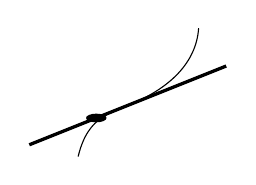
\begin{tikzpicture}[x=1cm,y=1cm]
\draw[line width=1.2pt] (0,0)--(2.5,1.0);
\draw (0.62,-0.15) .. controls (0.75,0.40) and (1.08,0.40) .. (1.25,0.50) .. controls (1.78,0.71) and (2.12,1.04) .. (2.15,1.48);
\fill (0.85,0.34) ellipse (0.13 and 0.055);
\end{tikzpicture}}

Considérons une \deleted{trivialisation} \inserted{base de $\mathcal E_3$ compatible avec} du drapeau \diagram{\begin{tikzcd}[column sep=small]0\arrow[rr,bend right=25]&\subset&\mathcal E_1\arrow[rr,bend right=25,dash]&\subset&\mathcal E_2\arrow[rr,bend right=25,dash]&\subset&\mathcal E_3\end{tikzcd}} de $\mathcal E_3$ \inserted{et commençant par $1_S\in\Gamma(S,\underline O_S)$;} [elle ``dépend de $(3+3-1)$ \inserted{$=5$} paramètres''], \deleted{par des coordonnées $z,y,x$} \inserted{i.e. une base $1,y,x$}

\margin{\diagram{$\left(\begin{array}{ccc}1&\alpha&\beta\\\diagdown&\mu&\sigma\\&\diagdown&\nu\end{array}\right)$}}

\deleted{Alors la forme $\varphi$ (définie à \unsure{unité} \deleted{\unsure{homothétie}} \inserted{multiplication près par \unsure{u}}) prend la forme [où on remplace $z$ par $1$]
\[
ax^{\unsure{2|3}}+by^3+cxy+dy^2+ex+fy+g=0
\]
\margin{$x^3\quad y^2$}
\inserted{où $y$ définit un \unsure{suppl.} de $\mathcal E_1$ dans $\mathcal E_2$ et $x$ de $\mathcal E_2$ dans $\mathcal E_3$}}

\mspage{8}

\scanpage{10}

\deleted{qui est aussi la relation (unique, \inserted{à \uline{unité près}}, \unsure{que vérifie aussi bien à priori}) \unsure{vérifiée par}} Puisque $1,y,x,y^2,xy,y^3$ forment une base de $\mathcal E_6$ (adaptée à la filtration) on aura donc une équation
\[
\varphi(x,y)=\boxed{x^2+ay^3+bxy+cy^2+dx+ey+f=0}
\]
\margin{\figure{\begin{tikzpicture}\node[draw,ellipse,inner sep=3pt] {$\Delta(a,b,c,d,e,f)\in L^{\otimes12}$};\end{tikzpicture}}}
qui est d'ailleurs une équation valable dans $\mathcal E_6$ considéré comme \unsure{composante de} $\Gamma_*(f,\underline L^{\otimes3})\simeq\coprod_{i\geq0}\mathcal E_i$, satisfaite entre les sections $x,y$ de $\mathcal E_3$ \deleted{\unsure{de même $\mathcal E_3$, $y^3$}}, \inserted{à valeurs en $\mathcal E_9$, \deleted{\unsure{$\mathcal E_3$}}}.

\deleted{Cette équation} Si on désigne par $z$ la section $1$ de $\mathcal E_0=\mathcal E_1\subset \mathcal E_3$, et qu'on \deleted{\unsure{la}} écrit \inserted{notre équation} sous la forme
\[
\Phi(x,y,z)=x^2z+ay^3\deleted{\unsure{z}}+bxyz+cy^2z+dxz^2+fz^3=0
\]
on \uline{constate alors} que $\Phi$ est la forme de degré $3$ qui définit \deleted{\unsure{notre}} $C$ dans $P(\mathcal E_3)\simeq P_S^3$. En effet si $\Phi'$ est la forme qui définit $C$, alors $\Phi$ est \uline{un multiple de $\Phi'$}, et \deleted{\unsure{d'une}} c'est un multiple par quelque chose qui est inversible, puisque $\Phi$ est ``non nulle'' en tt pt de $S$ --- un de ses coefficients est $1$ ---.
\margin{\unsure{d'ailleurs, est essentiellement primitive}}
\margin{préciser ce pt cf. intersections complètes}
\mspage{9}

\scanpage{11}

Réciproquement, partons d'une équation comme dessus, où les \deleted{$a$}\inserted{coeff. $a,b\ldots$} sont des sections de $\underline O_S$. On sait qu'\deleted{$a$}\inserted{une telle équation} définit un diviseur relatif \inserted{positif} de $P_S^2/S$, soit $C$. Il reste à écrire que c'est là une \uline{courbe simple} sur $S$. On sait qu'il faut pour cela que le discriminant de la forme
\[
\delta(a,b,c,d,e,f)
\]
soit une \uline{unité} partout. Ici le discriminant s'explicite : ---

On a obtenu en résumé

\uline{Proposition} La donnée d'une courbe elliptique sur $S$, \deleted{\unsure{avec}}\inserted{munie} d'une \deleted{``base adaptée''}\inserted{``base spéciale''} de $\mathcal E_3(C/S)$, \deleted{``unité''} est équivalente à la donnée de sections $a,b,c,d,e,f$ de $\underline O_S$ satisfaisant $\delta(a,b,c,d,e,f)\unsure{\neq|=}0$ ; cette correspondance est compatible avec l'image inverse.

On tire de ceci : Considérons le schéma affine de type fini sur $\mathbb Z$
\[
M=\operatorname{Spec}(\mathbb Z[A,B,C,D,E,F][\delta^{-1}])
\]
qui est un ouvert affine de $\operatorname{Spec}\mathbb Z[A,B,C,D,E,F]\simeq \unsure{\mathbb E|E}_{\mathbb Z}^6$. \deleted{Faisons opérer \unsure{dessus|dans}}
\mspage{10}

\scanpage{12}

\deleted{\unsure{puis schéma en groupes} $G$, de type fini sur $\mathbb Z$, qui \deleted{\unsure{repr.}} est représenté matriciellement par}

\unsure{$G$.} Considérons le schéma en groupes de $\operatorname{GL}(\unsure{n|3})_{\mathbb Z}$ qui correspond aux matrices de la forme
\diagram{\[\left(\begin{array}{ccc}1&\alpha&\gamma\\0&\lambda&\beta\\0&0&\mu\end{array}\right)\]}
(avec $\lambda\mu$ une unité bien sûr), \inserted{il opère sur $M$} de la façon évidente qui consiste à interpréter $ABCDEF$ comme coeff. d'une forme
\[
\deleted{\unsure{X^2}+AXY^2}\qquad X^2\unsure{+|-}AY^3+BXY^2+CY^{\unsure{3|2}}+DX+EY+F
\]
et en faisant sur $X,Y$, la substitution affine
\[
\unsure{Y|X}'=\lambda\unsure{Y|X}+\alpha,\quad X'=\mu X+\beta Y+\gamma
\]
[on peut aussi dire --- \unsure{ce sera plus clair}, que $G$ opère sur le \unsure{vecteur} $E_3$, donc dans $\Phi_3(E_3)$, et qu'il laisse invariant le sous-\deleted{module}\inserted{\unsure{schéma}} de \deleted{\unsure{dimension}}\unsure{rang} $6$ des formes qui sont de la forme dite, d'où les opérations de $G$ sur $M$.

\margin{\uuline{Prop}}
Mais le foncteur qui à tt $S$ attribue \unsure{l'ens.} \inserted{l'ens des classes à isom près} des courbes elliptiques ``structurées'' comme dessus sur $S$, est \uline{représentable} par $M$. De plus, pour que deux \unsure{éléments} de
\mspage{11}

\scanpage{13}

$M(S)$ définissent des courbes elliptiques isomorphes (non structurées) il faut que \deleted{\unsure{donc}} ils soient conjugués par une opération de $G(S)$, où \inserted{$G$ est un groupe \unsure{linéaire|lisse} sur $S$.} Enfin, pour tte courbe elliptique $C$ sur $S$, il existe une extension \deleted{fid. plat}\inserted{simple surj. de type fini} $S'$ de $S$ [savoir le fibré principal associé à $\mathcal E_3$ pour le \unsure{clivage} qu'on a mis sur $\mathcal E_3$] telle que \deleted{sur} $C_{S'}$ ``provienne'' d'un élément de $M(S')$.

Ainsi, avec une terminologie générale, le foncteur $F$ : ``classes à isom près de courbes elliptiques sur $S$'' est \deleted{\unsure{pro}}-$\mathcal D$-représentable, où $\mathcal D$ désigne la catégorie des morphismes simples surjectifs. Si ce n'était que pour \unsure{obtenir cet énoncé}, on n'aurait pas à se donner tant de mal, \uline{car} on a un raisonnement général qui le donne pour les courbes de genre $g$ \unsure{quelc} (de façon \unsure{triangulaire} \unsure{quotient} par un groupe projectif---).
\mspage{12}

\scanpage{14}

Une normalisation un peu plus poussée est obtenue ainsi : on se donne une trivialisation de $L$ par une section partout non nulle $D$ de $L$, [dérivation invariante], on choisit alors la base $1,x,y$ de $\mathcal E_3$ de façon que l'image de $y$ dans $L_2$ soit $i_2(D)$, celle de $x$ dans $L_3$ soit $i_3(D)$. \deleted{Cela}

\deleted{[} i.e. on prend comme structure auxiliaire la donnée d'un $\mathcal L$ \inserted{inv.}, d'un $\mathcal E$ loc. libre de rang $3$, muni d'un splitting \unsure{où} les facteurs successifs sont munis d'un isom avec $\mathcal L^0,\mathcal L^2,\mathcal L^3$ respectivement.
Le groupe d'automorphismes de cette structure est \deleted{\unsure{formé}} le sous-groupe de $G_m\times\operatorname{GL}(3)_S$, formé des \deleted{\unsure{triplets}}\inserted{couples} de la forme
\diagram{\[\left(\lambda,\left(\begin{array}{ccc}1&\alpha&\beta\\0&\lambda^2&\gamma\\0&0&\lambda^3\end{array}\right)\right)\]}
\[
\lambda\in\Gamma(G_{mS}/S)=\Gamma(S,\underline O_S^*)\qquad
\alpha,\beta,\gamma\in\Gamma(S,\underline O_S)
\]

\deleted{La fixation de la structure ainsi \unsure{conduit à une équation}} \inserted{isomorphe} \deleted{i.e.} \unsure{le} sous-groupe du \deleted{\unsure{précédent}}\inserted{groupe plein}
\diagram{\[\left(\begin{array}{ccc}1&\alpha&\beta\\0&\lambda&\gamma\\0&0&\mu\end{array}\right)\]}
pour
\[
\lambda=\left(\frac\mu\lambda\right)^2,\qquad
\mu=\left(\frac\mu\lambda\right)^3\qquad\text{i.e.}\quad\boxed{\mu^2-\lambda^3=0}.
\]

L'équation de $C$ pour une telle base \deleted{prend alors la forme} [caractérisée par la condition $\underline{x^2-y^3\in \mathcal E_5}$] prend la forme
\[
x^2-y^3+bxy+cy^2+dx+ey+f=0
\]
[i.e. on fait $a=-1$ en l'équation plus haut] \inserted{avec $\delta(b,c,d,e,f)$ une unité}
\mspage{13}

\scanpage{15}

Il ne semble pas qu'on puisse obtenir des normalisations locales sans \deleted{\unsure{type}} restriction de car. qui ferait intervenir moins de paramètres, [si on veut qu'elle soit subordonnée à la descente \deleted{\unsure{de}} par morphismes plats, ou \unsure{à|m.} simples]. Si on admet des ext. de base finies et plates, on peut pousser la normalisation plus loin en exigeant que $\delta(b,c,d,e,f)=1$ i.e. \inserted{(intrinsèquement)} se donner des trivialisations de $\unsure{\mathcal L|L}$ \deleted{compatibles} définies par des sections $\unsure{\lambda|D}$ dont la puissance $12$.ième (\unsure{ou même} $24$.ième) est \inserted{$\delta^{-1}$, où $\delta$ est} le discriminant. On va \deleted{\unsure{en ce}} donner des \deleted{\unsure{les}} normalisations plus poussées en car $\neq2$, puis en car. $\neq3$, puis on verra.
\mspage{14}

\scanpage{16}

Transformons l'équation
\[
x^2=y^3+\unsure{\dot a|a}xy+by^2+cx+dy+e
\]
par $s$, et en rappelant que $sx=-x$, $sy=y$, on trouve
\[
x^2=y^3\unsure{-|+}axy+by^2-cx+dy+e
\]
et en comparant on trouve $a=c=0$, donc l'équation ici se met sous la forme
\[
\boxed{x^{\unsure{2|3}}=y^{\unsure{3|2}}+ay^2+by+c}
\]
avec comme condition $\delta(a,b,c)\neq0$, qui ici ne fait qu'exprimer que les solutions de $P(y)=y^3+ay^2+by+c$ sont distinctes en tt pt de $S$.

\margin{\unsure{quotient}}
Géométriquement, \deleted{\unsure{le schéma}} l'équation s'interprète ainsi : le quotient $C/\mathbb Z_2$ est un schéma de \unsure{Brauer-Sévéri} \inserted{$P$} sur $S$, muni d'une section \unsure{marquée} (correspondant à la section nulle de $C$ sur $S$), donc \deleted{s'identifie} \deleted{est} \deleted{isomorphe}\inserted{canoniquement} à un espace principal homogène sous un \deleted{\unsure{faisceau inverse}} \deleted{fibré \unsure{qui est} loc. libre} \unsure{fibré vectoriel} \deleted{\unsure{de rang un}}\inserted{inversible} [il correspond à $L^{\otimes2}$]

$C$ est ramifié \deleted{et} au dessus d'un diviseur relatif \inserted{de $P/S$} étale sur $S$, qui se décompose en la section à l'infini, et en un diviseur relatif \inserted{de $P/S$} étale sur $S$, \deleted{\unsure{dans les fibres}} de \deleted{\unsure{$E$}} $\underline V(L^{\otimes2})/S$ étale sur $S$, de degré relatif $3$.
\mspage{15}

\scanpage{17}

\deleted{Supposons \unsure{que tous les corps résiduels de}}

Notons qu'il y a dans $C$ un $S$-automorphisme canonique de symétrie, car $C$ est un schéma abélien sur $S$. Cet automorphisme \inserted{est d'ordre $2$, il} opère sur les $\mathcal E_i$ [de façon compatible avec les structures, multiplications \inserted{et les opérations de $\mathcal L$ sur $\mathcal E_\infty$}] et induit sur $\mathcal L$ le chgt de signe.
\deleted{\unsure{Il en résulte aussitôt qu'il opère trivialement dans $\mathcal E_2$ [car il y opère trivialement]}}
\deleted{Si les caractéristiques résiduelles de $S$ sont $\neq2$, on en conclut}

Supposons les car. résiduelles de $S\neq2$. Alors
\deleted{Il existe un supplémentaire unique de $\mathcal E_1$ dans $\mathcal E_2$ \unsure{stable qui sera le lieu $s$ opère}}
$s$ opère trivialement dans $\mathcal E_2$ [c'est ainsi \unsure{sans|sous} la condition qu'on vient de faire, on le verra], et il existe un supplémentaire unique \inserted{$L_3$} de $\mathcal E_2$ dans $\mathcal E_3$ où $s$ opère par symétrie, \deleted{\unsure{le}} qui est aussi égal à $\mathcal L\cdot \mathcal E_2$, on le note $L_3$.
\margin{N.B. la \unsure{considération} de $C\longrightarrow P(\mathcal E_2)$ et de la \unsure{différentielle} de ce morphisme nous donne (sans restriction de car) un morphisme
\diagram{\begin{tikzcd}\unsure{\mathcal L|L}^{\otimes3}\arrow[r,"\unsure{\partial|\vartheta}"]&\mathcal E_3\end{tikzcd}}
\unsure{compatible avec tt changement de base $S$}.}

\deleted{Alors $L_3^{\otimes2}$ est un supplémentaire de $\mathcal E_5$ dans $\mathcal E_6$, soit $L_6$. A condition}
On peut donc normaliser encore plus les bases admissibles de $\mathcal E_3$, en exigeant que $x$ soit une base de $\unsure{\mathcal E_3|L_3}$ ; donc le groupe des changements de base admis est celui de la forme
\diagram{\[\left(\begin{array}{ccc}1&\alpha&0\\0&\lambda^2&0\\0&0&\lambda^3\end{array}\right)\qquad\text{i.e.}\qquad\left(\begin{array}{ccc}1&\alpha&0\\0&u&0\\0&0&v\end{array}\right)\]}
avec $\deleted{\unsure{\lambda}}u^3-v^2=0$.
Ce n'est autre que le \uline{groupe affine à $1$ variable}.

Quelle est la normalisation correspondante de l'équation de $C$ ?
\mspage{16}

\scanpage{19}

\figure{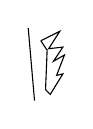
\begin{tikzpicture}[x=.4cm,y=.4cm]\draw (0,0)--(-.2,2.3);\draw (.2,1.9)--(.8,2.2)--(.45,1.65)--(.9,1.7)--(.6,1.25)--(.95,1.45)--(.7,.8)--(.9,.85)--(.5,.2)--(.35,.35)--(.4,1.6)--(.2,1.9);\end{tikzpicture}}
$b$

\uuline{$j$ et $j-1$ \unsure{unité}}

Cas $A$ \unsure{local} \uline{normal}
\[
\left\{\begin{array}{ll}
j\text{ une unité, pas }j-1,\ \unsure{(\text{par idéal})}&(1-j^{-1})^2\in A^6\unsure{A^*}\\
j-1\text{ une unité, }j\text{ pas}\ \unsure{(\text{par idéal})}&\left(\dfrac{\unsure{1|j}}{j-1}\right)^3\in A^6A^*
\end{array}\right.
\]

\figure{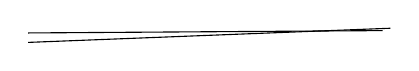
\begin{tikzpicture}\draw (0,0)--(4.5,.03);\draw (0,-.12)--(4.6,.06);\end{tikzpicture}}
\margin{\uline{à vérifier} \uline{\unsure{géométriquement}}}
\diagram{\begin{tikzcd}[column sep=large]
\text{Ext. Kummérienne de gr }\mathbb Z/3 \arrow[r,leftrightarrow]& j\equiv1
\end{tikzcd}}
\[
b^3=0,\quad c\text{ inversible}\quad //
\]
Si \deleted{\unsure{a}} $A$ \unsure{ss élémts nilpotts}, alors l'invariant
\[
c\in A^*/A^{*(\unsure{3|6})}.
\]
\diagram{\begin{tikzcd}[column sep=large]
\text{Ext. Kummérienne de gr }\unsure{Z|\mathbb Z}/2 \arrow[r,leftrightarrow]&j\equiv0
\end{tikzcd}}
\[
c^2=0,\quad b\text{ inversible}\quad //
\]
Si $A$ \unsure{ss élémts nilpotts} alors l'invariant est
\[
b\in A^*/A^{*(2)}.
\]
\hrulefill

\hfill $1-$

\figure{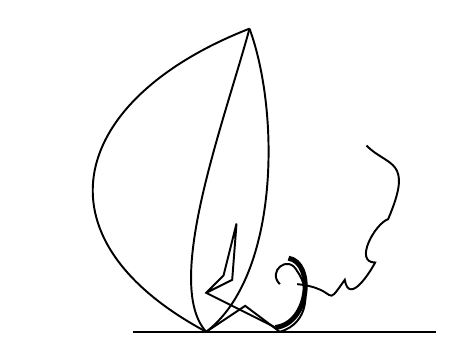
\begin{tikzpicture}[x=.55cm,y=.55cm,line width=.7pt]
\draw (-.6,0)--(6.4,0);
\draw (2.1,7) .. controls (-2,5.4) and (-3,2.2) .. (1.1,0) .. controls (2.8,1.3) and (2.8,5.1) .. (2.1,7);
\draw (2.1,7) .. controls (1.5,4.8) and (.1,1.1) .. (1.1,0);
\draw (1.1,0)--(2,.6)--(2.8,0) .. controls (3.5,.2) and (3.5,1) .. (3.2,1.4) .. controls (3,1.8) and (2.5,1.4) .. (2.8,1.1);
\draw[line width=1.8pt] (2.7,.1) .. controls (3.5,.2) and (3.6,1.6) .. (3,1.7);
\draw (1.1,.9)--(1.7,1.2)--(1.8,2.5)--(1.5,1.3)--(1.1,.9)--(2.7,.1);
\draw (3.2,1.1) .. controls (4.2,1) and (3.8,.5) .. (4.3,1.2) .. controls (4.4,.6) and (4.9,1.4) .. (5,1.6) .. controls (4.5,1.6) and (5,2.5) .. (5.3,2.6) .. controls (5.9,4) and (5.3,3.8) .. (4.8,4.3);
\end{tikzpicture}}
\[
\deleted{\unsure{j}}\quad\left(\frac{t}{t-1}\right)^3\in O^6O^*\qquad\uline{\unsure{\text{module}\ p|\text{unité}\ pr}}
\]
\[
\left(\frac{t-1}{t}\right)^2\in O^6O^*\qquad\text{``}\qquad
\sqrt[6]{\frac{t\deleted{\unsure{t}}}{t-1}}
\]
\hrulefill

\figure{
\begin{tikzpicture}[x=.7cm,y=.7cm]\draw[line width=3pt] (0,0) circle (.42);\end{tikzpicture}}
\[
\sqrt[2]{\frac{t}{t-1}}\qquad\sqrt[3]{\frac{t-1}{t}}\qquad \tfrac12\qquad\tfrac13
\]
\figure{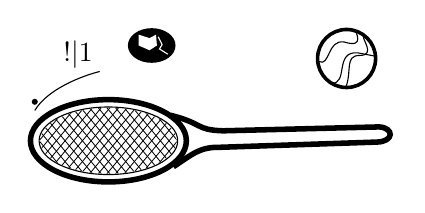
\begin{tikzpicture}[x=.55cm,y=.55cm]
\node at (-.7,2.2) {$\unsure{!|1}$};
\fill (1,2.4) ellipse (.55 and .4);
\fill[white] (.7,2.65)--(.95,2.57)--(1.1,2.65)--(1.12,2.4)--(.95,2.29)--(.7,2.4)--cycle;
\draw[white] (1.15,2.6)--(1.24,2.42)--(1.18,2.32)--(1.37,2.2);
\draw[line width=1.3pt] (5.5,2.1) circle (.67);
\draw (4.86,2.03) .. controls (5.12,1.9) and (5.05,2.55) .. (5.45,2.48) .. controls (5.95,2.32) and (5.68,2.75) .. (5.72,2.73);
\draw (5.15,1.53) .. controls (5.55,1.5) and (5.21,2.28) .. (5.76,2.23)--(6.13,2.16);
\draw (5.48,1.43) .. controls (5.63,1.81) and (5.45,2.17) .. (5.8,2.17) .. controls (6.2,2.17) and (5.82,2.58) .. (5.9,2.62);
\fill (-1.7,1.1) circle (.07);
\draw[line width=2pt] (0,.2) ellipse (1.8 and .95);
\draw (0,.2) ellipse (1.6 and .78);
\begin{scope}\clip (0,.2) ellipse (1.58 and .76);
\foreach \k in {-3,-2.8,...,3}{\draw[line width=.3pt] (\k,-1)--(\k+2,1.4);\draw[line width=.3pt] (\k,-1)--(\k-2,1.4);}\end{scope}
\draw[line width=2pt] (1.43,.79) .. controls (2.2,.6) and (2,.45) .. (2.65,.43)--(6.25,.52) .. controls (6.6,.5) and (6.6,.18) .. (6.2,.17)--(2.6,.05) .. controls (2.1,.06) and (1.96,-.1) .. (1.5,-.4);
\draw (-1.7,.9) .. controls (-1.4,1.4) and (-.6,1.7) .. (-.2,1.8);
\end{tikzpicture}}
\[
\lambda^{3/6}\cdot\lambda^{\unsure{-2/6}}=\lambda^{1/6}\qquad
\frac{-27c^{\unsure{2}}}{b^3-27c^2}=j
\]
\figure{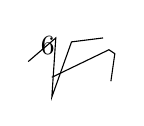
\begin{tikzpicture}[x=.5cm,y=.5cm]\node at (0,1) {$6$};\draw (-.5,.6)--(.2,1.2)--(.1,-.3)--(.6,1.1)--(1.4,1.2);\draw (.1,.2)--(1.55,.9)--(1.7,.8)--(1.6,.1);\end{tikzpicture}}
\[
s^6=\frac{t}{t-1}\qquad \frac{b^3}{c^2}=j\qquad 27c^2(j-1)=b^3j
\]
\diagram{\begin{array}{ccc}L&L^2&L^3\\&b&c\end{array}}
\[
b^{\deleted{\unsure{3}}}=27\frac{j-1}{j}\qquad
\boxed{\frac{b^3}{c^2}=27\frac{j-1}{j}}
\]
\figure{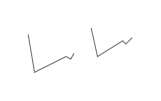
\begin{tikzpicture}[x=.4cm,y=.4cm]\draw[gray] (0,1.2)--(.2,0)--(1.2,.5)--(1.35,.42)--(1.45,.6);\draw[gray] (2,1.4)--(2.2,.5)--(3,1)--(3.1,.9)--(3.3,1.1);\end{tikzpicture}}
\figure{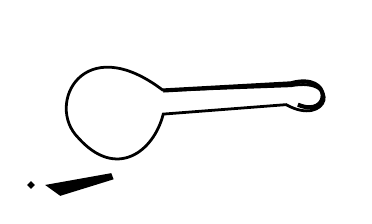
\begin{tikzpicture}[x=.6cm,y=.6cm,line width=1pt]\draw (0,0) .. controls (-1.7,1.3) and (-2.5,-.3) .. (-1.8,-1) .. controls (-1,-1.9) and (-.2,-1.3) .. (0,-.5)--(2.6,-.3) .. controls (3.5,-.8) and (3.8,.3) .. (2.7,.1)--(0,0);\draw[line width=1.5pt] (0,0)--(2.7,.15) .. controls (3.6,.4) and (3.55,-.6) .. (2.85,-.3);\fill (-2.5,-2)--(-1.1,-1.75)--(-1.05,-1.88)--(-2.18,-2.23)--cycle;\draw (-2.8,-2) circle (.04);\end{tikzpicture}}
\[
c=27\frac{j-1}{j}
\]
\deleted{\unsure{Hom}($\unsure{\widetilde E}$,)}
\[
f_*(\widetilde E)
\]
\diagram{\begin{tikzcd}
&\unsure{\underline{\mathrm H}|\underline{\mathrm{Hom}}}_{\unsure{O|0}}(E,\unsure{\underline O|\underline U})\\
\unsure{\underline{\mathrm H}|\underline{\mathrm{Hom}}}_{\underline A}(\widetilde E,\underline A)\times&\unsure{\underline{\mathrm H}|\underline{\mathrm{Hom}}}_{\underline O}(\underline A,\underline O)\arrow[u]
\end{tikzcd}}
\[
\boxed{x^3+27\frac{j-1}{j}(x+1)=0}
\]
\mspage{18}

\scanpage{20}
\mspage{19}

\figure{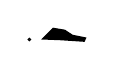
\begin{tikzpicture}[x=.5cm,y=.5cm]\draw (-.3,0) circle (.03);\fill (0,0)--(.3,.3)--(.6,.25)--(.8,.12)--(1.15,.05)--(1.1,-.06)--(.5,-.02)--cycle;\end{tikzpicture}}

\begin{center}$-\ 20\ -$\end{center}\hfill n\textsuperscript{o} 276

\S2. -- \uline{Anneaux} $\mathrm m$-\uline{adiques noethériens}.

Dans tout ce \S\ on désigne par $A$ un anneau \uline{commutatif noethérien} et par $\mathrm m$ un idéal de $A$ ; sauf mention explicite du contraire on munira $A$, et plus généralement tous les $A$-modules considérés, de la topologie $\mathrm m$-adique.

\figure{\begin{tikzpicture}[x=.5cm,y=.5cm]\draw[gray] (0,1) .. controls (-2,1.5) and (-3,-.5) .. (-.5,-.8) .. controls (.3,-.8) and (.7,-.2) .. (1.1,-.1);\draw (1.1,-.1)--(1.5,.05);\draw (2,-.1)--(4,-.1);\draw (2.3,.15)--(4,.15);\draw[gray] (.6,-1.3) circle (.35);\draw[gray] (-.25,-2.3) circle (.38);\end{tikzpicture}}

1. -- \uline{Restriction de la topologie} $\mathrm m$-\uline{adique à un sous-module}.

\uline{Théorème} 1 -- \uline{Soient} $E$ \uline{un} $A$-\uline{module de type fini et} $F$ \uline{un sous-module de} $E$. \uline{La topologie} $\mathrm m$-\uline{adique du} $A$-\uline{module} $F$ \uline{est induite par la topologie} $\mathrm m$-\uline{adique de} $E$.

Le théorème 1 sera une conséquence du résultat plus précis que voici :

\uline{Lemme d'Artin-Rees} \unsure{--} \uline{Soient} $A$ \uline{un anneau commutatif noethérien}, $\mathrm m$ \uline{un idéal de} $A$, $E$ \uline{un} $A$-\uline{module de type fini et} $F$ \uline{un sous-module de} $E$. \uline{Pour tout entier} $k$ \uline{suffisamment grand on a}
\[
\mathrm m^pE\cap F=\mathrm m^{p-k}(\mathrm m^kE\cap F)\qquad\uline{\text{pour tout}}\ p\geq k.
\]
Il suffit évidemment de prouver l'inclusion\qquad --
\[
\mathrm m^pE\cap F\subset\mathrm m^{p-k}(\mathrm m^kE\cap F),
\]
puisque l'inclusion opposée est triviale.

Pour cela considérons dans l'anneau de polynômes $A[X]$ le sous-anneau $A'$ formé des polynômes $\sum a_pX^p$ tels que $a_p\in\mathrm m^p$ pour tout $p$. Il est clair qu'en tant qu'algèbre sur $A$, $A'$ est engendré par les $a_iX$ où $a_i$ est un système de générateurs de $\mathrm m$ ; par suite $A'$ est un anneau noethérien, par ailleurs gradué.

Formons de même le $A[X]$-module
\[
E[X]=A[X]\underset{A}{\otimes}E
\]
des polynômes à coefficients dans $E$ ; en tant que $A'$-module, $E[X]$ contient le sous-module $E'$ formé des polynômes $\sum e_px^p$ tels que $e_p\in\mathrm m^pE$

\scanpage{21}

\deleted{$(x_1-x_2)(x_3$}
\[
\prod_{\unsure{i\ne j}}(x_i-x_j)=\prod_i\left(\frac{f(x)}{\unsure{x_j|x}-x_i}\right)_{x\to x_i}=\prod_i f'(x_i).
\]
\margin{\figure{\begin{tikzpicture}[x=1cm,y=1cm]
\node[anchor=west] at (0.3,1.5) {$ (\unsure{y|x}+u)^3+a(y+u)^2 $};
\node at (1.7,0.8) {$3u+a$};
\node at (1.7,0.1) {$u=-\dfrac a3$};
\draw (-0.1,2.0) .. controls (0.5,1.5) and (0.4,0.2) .. (0.9,-0.3) .. controls (1.4,-0.5) and (2.5,-0.5) .. (3.2,-0.4);
\end{tikzpicture}}}
\[
f(x_i)=
\]
\[
3x^2+2ax+b
\]
\[
(3x_1^2+2ax_1+b)(3x_2^2+2ax_2+b)(3x_3^2+2ax_3+b)
\]
Supposons \uuline{$a=0$} \unsure{on trouve}
\margin{$x_1x_2\quad x_2x_3\quad x_3x_1$\par $x_1x_2\ x_2x_3$}
\[
j=-\frac{27c^2}{\Delta}
\]
\[
\begin{aligned}
\Delta=\prod(3x_i^2+b)&=27(x_1x_2x_3)^2+9b\bigl(\sum(x_1x_2)^2\bigr)\\
&\quad+3b^2\sum x_i^2\ \unsure{\}}+b^3
\end{aligned}
\]
\[
\deleted{=27c^{\unsure{3|2}}+9b(b^2-2\sum x_1^2x_2x_3}
\]
\[
(x_1x_2x_3)^2=c^2
\]
\[
\sum(x_1x_2)^2=(\sum x_1x_2)^2-2\sum x_1^2x_2x_3\ \unsure{=}
\]
\[
\sum x_i^2x_2x_3=(\sum x_1^2)(\sum x_2x_3
\]
\[
\boxed{\Delta=\deleted{\unsure{9|4}}b^3-27c^2}\quad ?
\]
\margin{$x_1^2x_2^2+$}
\[
\prod 3x_i^2+b
\]
\[
\deleted{(\sum\unsure{x^2})^2}
\]
\[
\cdot\ 3\sum(x_1x_2)^2+(\sum x_1x_2)(\sum x_i^2)
\]
\[
\deleted{\unsure{x_1x_2}}\qquad\deleted{x_1x_2}
\]
\mspage{20}

\scanpage{22}
\mspage{21}

\begin{center}$-\ 9\ -$\end{center}\hfill n\textsuperscript{o} 276

\uline{Remarque} -- La réciproque du corollaire précédent est fausse ; cf. Exerc. N.

4. -- \uline{Modules filtrés complets}.

Soit $(E,E_n)$ un module filtré sur un anneau filtré $(A,A_n)$. Puisque la structure uniforme du groupe topologique $E$ est définie par un seul écart, il est clair que $E$ \uline{est complet si et seulement si toute suite de Cauchy, dans} $E$ \uline{est convergente}. Par ailleurs en vertu de l'inégalité
\[
d(x_p,x_q)\leqslant\underset{p\leqslant n\leqslant q-1}{\operatorname{Max}}d(x_n,x_{n+1}),
\]
on voit qu'une suite $(x_n)$ de points de $E$ vérifie le critère de Cauchy si et seulement si la suite $d(x_n,x_{n+1})$ tend vers $0$, i.e. si et seulement si la suite de terme général $y_n=x_{n+1}-x_n$ tend vers $0$ dans $E$. On en déduit :

PROPOSITION 4 -- \uline{Pour que le module filtré} $E$ \uline{soit complet, il faut et il suffit que toute série d'éléments de} $E$ \uline{dont le terme général tend vers} $0$ \uline{soit convergente}.

\uline{Corollaire} 1-- \uline{Soit} $(E,E_n)$ \uline{un module filtré complet}. \uline{Tout sous-module fermé de} $E$, \uline{muni de la filtration induite, est complet}. \uline{Tout module quotient de} $E$, \uline{muni de la filtration quotient est complet}.
\margin{\unsure{fait général} pour les top\unsure{.} métrisables\quad !\quad\figure{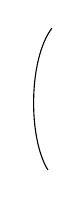
\begin{tikzpicture}[x=1cm,y=1cm]\draw (0.2,0.9) .. controls (-0.1,0.5) and (-0.1,-0.5) .. (0.15,-0.9);\end{tikzpicture}}}

L'assertion concernant les sous-modules \uline{résulte} trivialement de la Proposition. D'autre part, si l'on considère, dans un module quotient $E/F$ une série dont le terme général tend vers $0$, il est clair que celle-ci est l'image d'une série dans $E$ dont le terme général tend vers $0$, donc d'une série convergente dans $E$ ; l'application canonique $E\to E/F$ étant continue, $E/F$ est complet d'après la proposition 1.

\uline{Corollaire} 2 -- \uline{Soient} $(A,A_n)$ \uline{un anneau filtré et complet}, $E$ \uline{un} $A$-\uline{module de type fini}, \uline{filtré par les sous-groupes} $A_nE$. \uline{Alors} $E$ \uline{est complet}

Ecrivons $E=L/R$ où $L$ est un $A$-module libre de type fini ; la filtration de $E$ par les $A_nE$ se déduit alors de la filtration analogue de $L$ ;

\scanpage{23}

\[
\frac{(t+1)(2t-1)(t-2)}{t(t-1)}\unsure{=-|=}\frac{(2x_1\unsure{-}x_2-x_3)(2x_2-x_3-x_1)(2x_3-x_1-x_2)}{(x_1-x_2)(x_2-x_3)(x_3-x_1)}.
\]
\deleted{$\unsure{x_1x_2x_3}$}
\[
\boxed{j=-\frac1{27\Delta}\bigl[(2x_1-x_2-x_3)(2x_2-x_3-x_1)(2x_3-x_1-x_2)\bigr]^2}
\]
\margin{\[
\sum x_1=-a\qquad\sum x_1x_2=b\qquad x_1x_2x_3=\unsure{-}c
\]}
\[
\Delta=\bigl((x_1-x_2)(x_2-x_3)(x_3-x_1)\bigr)^2
\]
\[
j=\frac{\bigl[(3x_1+a)(3x_2+a)(3x_3+a)\bigr]^2}{-27\Delta}
\]
\[
\deleted{\frac{27}{-\Delta}\bigl[(a/3+x_1)(a/3+x_2)(a/3+x_3)\bigr]^2}
\]
\[
\deleted{\unsure{(a/3)}}
\]
\[
\begin{aligned}
\sqrt{-27\Delta j}&=a^3+3a^{\unsure{2}}(x_1+x_2+x_3)+9a(x_1x_2+x_2x_3+x_3x_1)\\
&\quad+27\deleted{\unsure{a}}x_1x_2x_3\\
&=a^3-3a^3+9b-27\deleted{\unsure{a}}c\\
&=-2a^3+9ab-27c
\end{aligned}
\]
\[
\boxed{j=\frac{(27c+2a^3-9ab)^2}{-27\Delta}}
\]
\[
\deleted{\prod(x_1^2+x_2^2-2x_1x_2)\unsure{=}}
\]
\mspage{22}

\scanpage{24}

\begin{center}$-\ 10\ -$\end{center}\hfill n\textsuperscript{o} 276

en vertu du corollaire précédent on peut donc se ramener au cas où $E$ est \uline{libre}, i.e. est produit direct d'un nombre fini de facteurs isomorphes à $A$. Raisonnant par récurrence, on est alors ramené à établir que si deux modules $E$ et $F$ (munis des filtrations associées à la filtration de $A$) sont complets il en est de même du module $E\times F$ ; or les relations
\[
A_pE\times A_qF\subset A_n(E\times F)\subset A_nE\times A_nF\qquad(p,q\leqslant n)
\]
montrent que $E\times F$ est le produit direct des groupes \uline{topologiques} $E$ et $F$. il est donc complet si $E$ et $F$ le sont.

PROPOSITION 5 -- \uline{Soient} $A$ \uline{un anneau commutatif}, $\mathrm m$ \uline{un idéal de} $A$, \uline{et supposons l'anneau} $A$ \uline{séparé} (resp. complet) \uline{pour la topologie} $\mathrm m$-\uline{adique}. \uline{Alors l'anneau de séries formelles} $A[[X]]$, \uline{filtré par les puissances de l'idéal} \inserted{\unsure{engendré}} \uline{par} $\mathrm m$ \uline{et} $X$, \uline{est séparé} (resp. \uline{complet}).
\margin{\unsure{Dire que la} \unsure{top. est} \unsure{celle de} la \unsure{conv. simple} des coefficients.}

Soit $\mathrm n$ l'idéal de $B=\unsure{'}A[[X]]$ engendré par $\mathrm m$ et $X$ : c'est l'ensemble des séries formelles $\sum a_nX^n$ telles que $a_0\in\mathrm m$. On déduit de là que pour tout entier $p$, l'idéal $\mathrm n^p$ est formé des séries $\sum a_nX^n$ telles que l'on ait $a_n\in\mathrm m^{p-n}$ pour $0\leqslant n\leqslant p$. Il résulte immédiatement de là que $B$ est séparé si $A$ est séparé. Supposons de plus $A$ complet, et considérons dans $B$ une série $\sum y_i$ dont le terme général
\[
y_i=\sum a_{in}X^n
\]
tend vers $0$ ; pour tout entier $p$ on a donc
\[
(1)\qquad a_{in}\in\mathrm m^{p-n}\qquad(0\leqslant n\leqslant p)\text{ pour }i>i_p.
\]
En fixant $n$ et en faisant varier $p$ on voit, puisque $A$ est complet, que la série $\sum_i a_{in}$ converge dans $A$ ; soit $a_n$ l'une des ses sommes (on ne suppose pas $A$ séparé). En vertu de (1) et du fait que les puissances de $\mathrm m$ sont fermées dans $A$, on a, quels que soient $n$ et $p\geqslant n$, la relation
\[
\sum_{i>i_p}\unsure{a_{in}|e_{in}}\in\mathrm m^{p-n}
\]
\mspage{23}

\scanpage{25}

\[
y^2=4x^3-h(x+1)\qquad h=27j(j-2^6 3^3)^{-1}
\]
\[
\deleted{y^2=\unsure{a}x^3+bx^{\unsure{2}}+cx+d}
\]
\diagram{\begin{array}{ccccccc}y^2=x^3+&ax^2&+&bx&+&c\\&1&&2&&3\end{array}}
\diagram{\begin{tikzcd}x_1\arrow[d]&x_2\arrow[d]&x_3\arrow[d]&\unsure{x_4}\arrow[d]\\\infty&0&1&t\end{tikzcd}}
\diagram{\begin{tikzcd}[column sep=small]
\infty\arrow[rrr,no head,to path={(\tikztostart.north)--([yshift=12pt]\tikztostart.north)--([yshift=5pt]\tikztotarget.north)--(\tikztotarget.north)\tikztonodes}]\arrow[rr,no head,to path={(\tikztostart.south)--([yshift=-8pt]\tikztostart.south)--([yshift=-8pt]\tikztotarget.south)--(\tikztotarget.south)\tikztonodes}]
&0\arrow[rr,no head,to path={(\tikztostart.north)--([yshift=5pt]\tikztostart.north)--([yshift=5pt]\tikztotarget.north)--(\tikztotarget.north)\tikztonodes}]\arrow[r,no head,to path={(\tikztostart.south)--([yshift=-4pt]\tikztostart.south)--([yshift=-4pt]\tikztotarget.south)--(\tikztotarget.south)\tikztonodes}]&1&t
\end{tikzcd}}
\diagram{\begin{tikzcd}[column sep=0pt]
((0,\arrow[rrr,no head,to path={(\tikztostart.south)--([yshift=-7pt]\tikztostart.south)--([yshift=-7pt]\tikztotarget.south)--(\tikztotarget.south)\tikztonodes}]
&1,\arrow[rr,no head,to path={(\tikztostart.south)--([yshift=-7pt]\tikztostart.south)--([yshift=-7pt]\tikztotarget.south)--(\tikztotarget.south)\tikztonodes}]&\infty,&t))&=((x_{\unsure{1}},x_{\unsure{2}},x_{\unsure{3}},x_4))
\end{tikzcd}}
\[
\begin{aligned}
\frac{x_1-x_3}{x_1-x_4}:\frac{x_2-x_3}{x_2-x_4}&=\frac{0-\infty}{0-t}:\frac{1-\infty}{1-t}\\
&=\frac{1-t}{-t}=-\frac1t+1
\end{aligned}
\]
\[
\frac{t-1}{t}\qquad\frac{t-\infty}{t-0}:\frac{1-\infty}{1-0}
\]
\deleted{$\unsure{x_3}$}
\[
t=\frac{1-\infty}{1-0}:\frac{t-\infty}{t-0}=\frac{x_3-x_1}{x_3-x_2}:\frac{x_4-x_1}{x_4-x_2}
\]
Si $x_4=\infty$, \unsure{on trouve}
\[
\boxed{t=\frac{x_3-x_1}{x_3-x_2}}\qquad t-1=\frac{x_2-x_1}{x_3-x_2}
\]
\margin{\[
\frac{c-a}{c-b}\ \Big|\ \frac{c-b}{c-a}\qquad
\frac{a-b}{c-b}\unsure{=|\cdot}\frac{b-a}{b-c}
\]
\diagram{\begin{tikzcd}\dfrac{a-b}{a-c}\arrow[loop right,no head,to path={([xshift=-12pt,yshift=8pt]\tikztostart.north)--([xshift=12pt,yshift=8pt]\tikztostart.north) .. controls ([xshift=18pt,yshift=8pt]\tikztostart.north) and ([xshift=18pt,yshift=2pt]\tikztostart.north) .. ([xshift=18pt]\tikztostart.north)--([xshift=18pt,yshift=-10pt]\tikztostart.south)\tikztonodes}]\end{tikzcd}}}
\[
t+1=\frac{2x_3-x_1-x_2}{x_3-x_2}
\]
\[
2t-1=\frac{x_3-2x_1+x_2}{x_3-x_2}
\]
\[
t-2=\frac{-x_3-x_1+2x_2}{x_3-x_2}
\]
\mspage{24}

\scanpage{26}

\figure{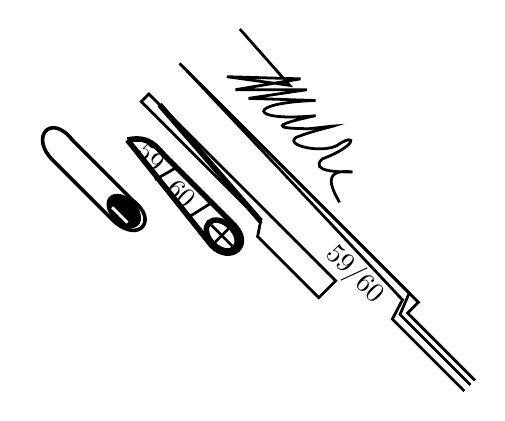
\begin{tikzpicture}[x=.55cm,y=.55cm,line width=1pt]
\begin{scope}[rotate=-45]
\draw (0,1)--(7.5,1)--(7.7,.5)--(10,.5);\draw (.25,1)--(7.5,.78)--(7.65,.3)--(10,.3);\draw (.65,1)--(7.8,1)--(7.8,.65)--(10,.65);
\draw (0,0)--(6.1,0)--(6.1,-.55)--(4.1,-.55)--(3.9,-.25)--(0,-.25)--cycle;
\draw[line width=2pt] (.35,0)--(3.9,-.25);\node[rotate=-45] at (6.3,.4) {$59/60$};
\draw[line width=2pt] (.4,-1.1) .. controls (.7,-.65) and (1,-.75) .. (1.3,-.75)--(3.5,-.75) .. controls (4.2,-.75) and (4.1,-1.45) .. (3.5,-1.45)--(.4,-1.1);
\draw (1.65,-.75)--(1.5,-1.3);\draw (2.8,-.75)--(2.65,-1.4);
\node[rotate=-45] at (1.05,-1) {$\unsure{59}$};\node[rotate=-45] at (2.15,-1.1) {$60$};
\draw[line width=2pt] (3.5,-1.12) ellipse (.42 and .28);\draw (3.15,-1.12)--(3.85,-1.12);\draw (3.5,-.86)--(3.5,-1.38);
\draw[line width=1.3pt] (-.5,-2) .. controls (-1.3,-1.9) and (-1.25,-2.65) .. (-.5,-2.65)--(1.5,-2.65) .. controls (2.3,-2.6) and (2.2,-1.9) .. (1.5,-2)--cycle;
\fill (1.5,-2.32) ellipse (.47 and .31);\draw[white] (1.25,-2.45)--(1.75,-2.45);
\end{scope}
\draw (2.1,1.5)--(3.25,.2)--(1.8,.4)--(3.5,.35)--(2,.1)--(3.65,.1)--(2.3,-.1)--(3.85,-.15) .. controls (2.2,-.2) and (2.3,-.65) .. (3.85,-.5) .. controls (2.9,-.7) and (2.8,-.8) .. (3.7,-.8) .. controls (4.7,-.7) and (4.2,-.7) .. (3.4,-1) .. controls (3.1,-1.2) and (4.1,-1.4) .. (4.4,-1.15) .. controls (4.8,-.9) and (4.8,-1.2) .. (4,-1.5) .. controls (3.7,-1.8) and (4.4,-1.8) .. (4.7,-1.8) .. controls (3.9,-1.7) and (4.3,-2.3) .. (4.4,-2.5);
\end{tikzpicture}}

\begin{center}$-\ 11\ -$\end{center}\hfill n\textsuperscript{o} 276

et par conséquent :
\[
a_n-\sum_{i=0}^{i=i_p}a_{in}\in\mathrm m^{p-n}.
\]
Considérant alors la série formelle $y=\sum a_nX^n$, la relation précédente montre que l'on a
\[
y-\sum_{i=0}^{i=i_p}y_i\in\mathrm n^p
\]
ce qui prouve que la série $\sum y_i$ converge vers $y$, d'où la proposition.

\uline{Corollaire} -- \uline{Soit} $A$ \uline{un anneau commutatif}. \uline{L'anneau de séries formelles} $A[[X_1,\ldots,X_r]]$ \uline{filtré par les puissances de l'idéal} $(X_1,\ldots X_r)$, \uline{est séparé et complet}.

5. -- \uline{Modules de type fini sur un anneau filtré complet}.

Soient $(E,E_n)$ et $(F,F_n)$ deux modules filtrés sur un anneau filtré $(A,A_n)$ par un \uline{homomorphisme} $u:(E,E_n)\longrightarrow(F,F_n)$ on entendra tout homomorphisme $u:E\longrightarrow F$ de $A$-modules, tel que l'on ait
\[
u(E_n)\subset F_n
\]
pour tout $n$. Si les filtrations de $E$ et $F$ sont associées à la filtration donnée de $A$, tout homomorphisme de $A$-modules est un homomorphisme de modules filtrés.

Il est clair que tout homomorphisme $u:(E,E_n)\longrightarrow(F,F_n)$ définit canoniquement un homomorphisme $G(u):G(E)\longrightarrow G(F)$ des $G(A)$-modules gradués associés, obtenu par passage au quotient.

PROPOSITION 6 -- \uline{Soient} $(E,E_n)$ \uline{et} $(F,F_n)$ \uline{deux modules filtrés sur un anneau filtré}, \uline{et} $u:(E,E_n)\longrightarrow(F,F_n)$ \uline{un homomorphisme de modules filtrés}. \uline{Supposons remplies les conditions suivantes} :

a) : $(E,E_n)$ \uline{est complet}.

b) : $(F,F_n)$ \uline{est séparé}.

c) : \uline{l'homomorphisme associé} $G(u)$ \uline{est surjectif}.
\mspage{25}

\scanpage{28}

$P^1_S$ sections $0,1,\infty$. Le groupe des automorphismes s'identifie au groupe $\mathfrak S_3$ des permutations des trois \unsure{pts} $0,1,\infty$, groupe à $6$ éléments $1,\varphi,\psi,\lambda,\mu,\nu$.
\[
(1)\quad\left\{\begin{array}{l}\varphi(t)=1-\dfrac1t\\\psi(t)=\dfrac1{1-t}\end{array}\right.
\qquad\text{2 permutations circulaires non triviales de }0,1,\infty
\]
\[
(2)\quad\left\{\begin{array}{ll||l}
\lambda t=\dfrac1t&\text{transposition de }0,\infty&1\\
\mu t=1-t&\text{transposition de }0,1&\infty\\
\nu t=1+\dfrac1{t-1}=\dfrac t{t-1}&\text{transposition de }1,\infty&0
\end{array}\right.
\]
\margin{\unsure{renommer}\quad
\[\left\{\begin{array}{l}\lambda t=1-\unsure{t}\\\mu t=\dfrac t{\unsure{t-1}}\\\nu t=\unsure{1/t}\\?\ ?\end{array}\right.\]}
\[
3\ a)\quad\boxed{\begin{array}{ll}\varphi^2=\psi&\psi^2=\varphi\\\deleted{\unsure{\psi^2=\varphi|\varphi^2=\psi}}&\varphi\psi=\psi\varphi=1\end{array}}
\]
\[
b)\quad\boxed{\lambda^2=\mu^2=\nu^2=1}
\]
\[
c)\quad\boxed{\begin{array}{l}\lambda\mu=\mu\nu=\nu\lambda=\varphi\\\mu\lambda=\nu\mu=\lambda\nu=\psi\end{array}}
\]
\diagram{\begin{array}{c}\displaystyle d)\quad\boxed{\begin{array}{l|l}\varphi\lambda=\mu\varphi=\nu&\psi\nu=\mu\psi=\lambda\\\varphi\mu=\nu\varphi=\lambda&\psi\mu=\lambda\psi=\nu\\\varphi\nu=\lambda\varphi=\mu&\psi\lambda=\nu\psi=\mu\end{array}}\end{array}}

$1,\varphi,\psi$ \unsure{gr. gr. cyclique} d'ordre $3$, de générateurs $\varphi$ et $\psi$, invariant dans $\mathfrak S_3$. Le quotient est $\mathbb Z/2$ et $\mathfrak S_3$ est produit semi-direct ; il y a trois sous-groupes sections, engendrés resp\unsure{\textsuperscript{t}} par $\lambda,\mu,\nu$ (leurs seuls éléments d'ordre $2$)
\[
4)\quad\left\{\begin{array}{lll}\varphi_\lambda=\mu&\varphi_\mu=\nu&\varphi_\nu=\lambda\\\psi_\nu=\mu&\psi_\mu=\lambda&\psi_\lambda=\nu\end{array}\right.
\]
\[
5)\quad\left\{\begin{array}{l}\lambda_\varphi=\mu_\varphi=\nu_\varphi=\psi\\\lambda_\psi=\mu_\psi=\nu_\psi=\varphi\end{array}\right.
\]
De plus, on a dans $P^1$ un automorphisme $\sigma$ \deleted{\unsure{de}} de carré $1$, donné par
\[
6)\quad\sigma t=\frac{t-2}{2t-1}\qquad[\sigma^2=\mathrm{id}]
\]
\unsure{permutant à} : $\unsure{\mathfrak S_6|\mathfrak S_3}$ (c'est d'ailleurs le seul, \unsure{sauf|avec}
\mspage{27}

\scanpage{29}
\mspage{28}

\begin{center}$-39-$\end{center}\hfill n\textsuperscript{o} 272

Corollaire 1.-- \uline{Pour toute famille} $a_i\in A_i$ $(1\leqslant i\leqslant n)$, \uline{il existe} $x\in B$ \uline{tel que} $x\equiv a_i\ (\mathrm{mod.}\ \underline{\mathrm p}_i)$.

Puisque les $\underline{\mathrm p}_i$ sont des idéaux maximaux de $B$, on a $B_{\underline{\mathrm p}_i}/\underline{\mathrm p}_iB_{\underline{\mathrm p}_i}=B/\underline{\mathrm p}_i$, et l'on peut donc supposer que $a_i\in B$ pour tout $i$. Dans ce cas, le corollaire signifie que l'application $B\longrightarrow\prod B/\underline{\mathrm p}_i$ est surjective, ce qui est un résultat bien connu (cf.Ch.I, \S2, cor. à la prop.4).

Corollaire 2.-- \uline{Il existe des éléments} $x_i\in K$ \uline{tels que} $v_i(x_i)=0$ \uline{et} $v_j(x_i)>0$ \uline{pour} $i\ne j$.

Pour chaque indice $i$, on applique le cor.1 à la famille $a_j=0$ si $j\ne i$, $a_i=1$.

Corollaire 3.-- \uline{Tout anneau de valuation contenant} $B$ \uline{contient l'un des} $A_i$.

Soit $A$ un anneau de valuation contenant $B$, et soit $\underline{\mathrm p}=\underline{\mathrm m}(A)\cap B$; il existe un idéal maximal $\underline{\mathrm p}_i$ de $B$ contenant $\underline{\mathrm p}$, d'où $A_i=B_{\underline{\mathrm p}_i}\subset B_{\underline{\mathrm p}}\subset A$.

[En fait, on a $A=B_{\underline{\mathrm p}}$ en vertu de la prop.1, mais on s'en fout.]

2. \uline{Valuations indépendantes}.

Définition 1.-- \uline{Soient} $A$ \uline{et} $A'$ \uline{deux anneaux de valuation d'un même corps} $K$. \uline{On dit que} $A$ \uline{et} $A'$ \uline{sont indépendants s'il n'existe aucun sous-anneau de} $K$, \uline{distinct de} $K$, \uline{les contenant}.

Bien entendu, on dit que deux valuations $v$ et $v'$ de $K$ sont \uline{indépendantes} si leurs anneaux sont indépendants.

\uline{Exemple}. Si $A$ et $A'$ sont \uline{distincts} et sont tous deux des anneaux de valuation de \uline{rang} $1$, ils sont indépendants, en vertu de la prop.7 du \S4.

Proposition 3.-- (\uline{théorème d'approximation}). \uline{Soient} $v_i$ $(1\leqslant i\leqslant n)$ \uline{des valuations deux à deux indépendantes d'un corps} $K$, \uline{et soient} $\Gamma_i$ \uline{leurs groupes des ordres}. \uline{Soient} $a_i\in K$ \uline{et} $\gamma_i\in\Gamma_i$ $(1\leqslant i\leqslant n)$. \uline{Il existe alors} $x\in K$ \uline{tel que} $v_i(x-a_i)\geqslant\gamma_i$ \uline{pour tout} $i$.

\scanpage{30}
\mspage{29}

l'identité). Il transforme $0,1,\infty$ en
\[
7)\quad\left\{\begin{array}{l}\sigma0=2\\\sigma1=-1\\\sigma\infty=\tfrac12\end{array}\right.
\]
\margin{Prouver : le normalisateur de $\mathfrak S_3$ dans $\operatorname{Aut}P^1_S$ est $\mathfrak S_3\times(\unsure{\mathbb Z}/2)$}

La différente de $\mathfrak S_3$ -- ou ens pts de ramification -- est \unsure{formé} des ens. des pts \unsure{de} un des cinq opérateurs $\lambda\mu\nu\varphi\psi$ \unsure{distincts} de l'identité. Pour $\lambda,\mu,\nu$ on trouve les sections $(\unsure{1},-1)(\infty,\tfrac12)(\unsure{\infty|0},2)$ ; [\unsure{st.ble} par $\sigma$]. Pour $\varphi$ (et $\psi$, c'est pareil), on trouve $1-\frac1t=t$ ou
\[
8)\qquad t^2-t+1=0
\]
i.e. l'équation cyclotomique
\[
\boxed{\Phi_6(t)=0}.
\]
\deleted{\unsure{Le}}

\deleted{\unsure{distinct de $\sigma$}}

C'est aussi l'\unsure{ens.} $\overline S$ des pts fixes de $\sigma$.

[Il est non ramifié \inserted{sur $S$} aux pts $s\in S$ tels que $k(s)$ soit de car. $\ne2,3$.].
\[
\mathbb Z_2=\mathfrak S_3/(\mathbb Z/3)
\]
y opère, de façon \uline{non triviale} aux pts où il est non ramifié sur $S$.

D'autre part, le schéma \inserted{$G$} des automorphismes de $P^1$ qui laissent $\overline S$ \unsure{globalement} invariant est une extension de $\mathbb Z_2$ [automorphismes de $\overline S$] par $(G_m)_S$ \uline{tordu} ---- [par le rev. cyclotomique]
\margin{\unsure{les except\textsuperscript{ns} qu'il y a pour car. $2$ ou $3$ de $S$}\quad\figure{\begin{tikzpicture}\draw (0,0)--(0,1.6);\end{tikzpicture}}}

\scanpage{31}
\mspage{30}

\begin{center}$-\ 47\ -$\end{center}\hfill n\textsuperscript{o} 272

$n=[L:K]$.\quad b) \uline{L'intersection} $B$ \uline{des} $A_i$ \uline{est la clôture intégrale de} $A$ dans $L$.

c) \uline{Si l'on pose} $\underline{\mathrm p}_i=B\cap\underline{\mathrm m}(A_i)$, \uline{les idéaux} $\underline{\mathrm p}_i$ \uline{sont des idéaux maximaux de} $B$, \uline{distincts} ; \uline{tout idéal maximal de} $B$ \uline{est égal à l'un des} $\underline{\mathrm p}_i$ \uline{et l'on a}
\[
A_i=B_{\underline{\mathrm p}_i}.
\]
Nous noterons $v_i$ (resp.$v$) des valuations associées aux $A_i$ (resp. à $A$), et $\Gamma_i$ (resp.$\Gamma$) les groupes des ordres correspondants. Le groupe $\Gamma$ s'identifie à un sous-groupe de chacun des groupes $\Gamma_i$.

Montrons d'abord que l'on ne peut pas avoir $A_i\supset A_j$ si $i\ne j$. En effet, d'après ce que l'on a vu au \S4, le groupe $\Gamma_i$ s'identifierait à un groupe quotient $\Gamma_j/H$, où $H$ est un sous-groupe isolé de $\Gamma_j$ ; puisque l'application canonique $\Gamma\longrightarrow\Gamma_j\longrightarrow\Gamma_j/H=\Gamma_i$ est une injection, on a $\Gamma\cap H=\{0\}$ dans $\Gamma_j$, ce qui montre que $H$ est isomorphe à un sous-groupe de $\Gamma_j/\Gamma$ ; comme ce dernier groupe est fini (prop.1), on a $H=0$, et les valuations $v_i$ et $v_j$ sont équivalentes, d'où $A_i=A_j$ contrairement à l'hypothèse $i\ne j$.

Montrons maintenant que le nombre des $A_i$ est \unsure{'} $\leqslant n$. Supposons donc qu'il existe $s$ anneaux $A_i$ distincts, avec $s>n$. D'après le cor. 2 à la prop.2 du \S6, (qui est applicable, en vertu de ce que l'on vient de voir), il existe des éléments $x_i\in L$, $1\leqslant i\leqslant s$, tels que $v_i(x_i)=0$ et $v_j(x_i)>0$ pour $i\ne j$. Montrons que les $x_i$ sont linéairement indépendants sur $K$, ce qui fournira la contradiction cherchée. Supposons que l'on ait une relation linéaire non triviale :
\[
\sum a_ix_i=0,\text{ avec }a_i\in K.
\]
Soit $a_j$ celui des $a_i$ dont la valuation est minimum ; quitte à multiplier les $a_i$ par $a_j^{-1}$ on peut supposer que $a_j=1$. On a alors une relation :

\scanpage{32}
\diagram{\begin{tikzcd}
e \arrow[r,no head] & G_m^{\text{tordu}} \arrow[r] & G \arrow[r] & \mathbb Z/2 \arrow[r] \arrow[d,equal] & e \\
e \arrow[r] & \mathbb Z/3 \arrow[u] \arrow[r] & \mathfrak S_3 \arrow[r] & \mathbb Z/2 \arrow[r] & e
\end{tikzcd}}

On suppose tjrs qu'il n'y a pas de pt $s$ de car. 2 ou 3 dans $S$. Alors \deleted{$\unsure{\mathfrak S_3}$ opère} $\mathfrak S_3\times \unsure{Z|\mathbb Z}_2$ opère ``tamely'' sur $P^1_S$ [en fait, il est compatible avec la fibration $P^1_S\to S$, et opère ``tamely'' sur les fibres\ldots] Le quotient \inserted{par un groupe ou un ss-groupe} \deleted{\unsure{il est|qui est}} \inserted{\unsure{est isomorphe}} encore à $P^1_S$ [car il est \uline{lisse} sur $S$, et rationnel sur $S$ d'après Lüroth]. Les schémas de pts fixes $(0,1,\infty)$ $(2,-1,\tfrac12)$ $(\bar S=x',x'')$ --- qui sont disjoints, et chacun stable sous $\mathfrak S_3$, qui \deleted{\unsure{y}} \inserted{lui-même} opère de façon \deleted{\unsure{simplement}} transitive sur chaque fibre, donnent dans $P^1_S/\mathfrak S_3$ trois \uline{sections} distinctes [à expliciter\ldots] qu'on peut utiliser pour identifier $P^1_S/\mathfrak S_3$ à $P^1_S$ avec les sections $\infty,0,1$. De même, \deleted{\unsure{le schéma du revt}} $P^1_S/(\mathbb Z/3)$ est muni d'abord de deux sections qui correspondent à $(0,1,\infty)$ et $(2,-1,\tfrac12)$, et qui
\mspage{31}

\scanpage{33}
\begin{center}- 46 -\end{center}
\hfill n$^\circ$ 272

l'application identique $k\longrightarrow k$, on a $\Omega\ne\unsure{\varnothing}$. Soit $(F,\psi)$ un élément maximal de $\Omega$. Montrons d'abord que $L$ est \uline{algébrique} sur $F$ ; sinon, en effet, il existerait $X\in L$ transcendant sur $F$, et $L$ contiendrait $F'=F(X)$ ; en composant la place $\lambda:F(X)\longrightarrow F$ donné par $f\longrightarrow f(0)$ avec la place $\psi:F\longrightarrow k$, on obtiendrait une place de $F'$ qui serait l'identité sur $k$, contrairement au caractère maximal de $(F,\psi)$. Donc $L/F$ est algébrique. Soit Alors $\psi'$ une place de $L$ à valeurs dans une extension $k'$ de $k$ qui prolonge $\psi$ ; une telle extension existe d'après la prop.4 du \S\ 2 ; en vertu de la prop.3, ci-dessus, $\psi'(L)$ est algébrique sur $\psi(F)=k$, donc $\psi'(L)=k$, \unsure{pui sque} $k$ est algébriquement clos, et la place $\psi'$ est la place cherchée.

[Ce n$^\circ$ pourrait remonter bien plus tôt à condition de donner une démonstration directe de la prop.3, ce qui n'est pas bien difficile. Est-ce que cela en vaut la peine ? La prop.4 est un résidu des rédactions antérieures (où elle était démontrée en même temps que le th. d'extension des valuations) ; le rédacteur ne pense pas qu'elle ait jamais servi à quoi que ce soit, et ne l'a gardée que sur les instances de Samuel ; il laisse à son Maître le soin de décider son sort (de la proposition, pas de Samuel)]

\unsure{3$^\circ$|3} - \uline{Prolongements d'une valuation à une extension algébrique}.

Soit $L$ une extension finie de $K$, dedegré $n$, et soit $A$ un anneau de valuation de $K$. Chercher les anneaux de valuation $A'$ de $L$ tels que $A'\cap K=A$ revient à chercher les prolongements d'une valuation $v$ associée à $A$ en une valuation $v'$ de $L$ (le groupe des ordres de $v'$ contenant celui de $v$ comme sous-groupe).

PROPOSITION 5 - \uline{Les anneaux de valuation} $A_i$ \uline{de} $L$ \uline{tels que} $A_i\cap K=A$ \uline{sont en nombre fini}. \uline{De plus} : a) \uline{leur nombre} $r$ \uline{est compris entre} 1 \uline{et}
\mspage{32}

\scanpage{34}
sont les sections de \unsure{ramification} de $P^1_S$ sur $P^1_S/(\mathbb Z/3)$. Passant au revêtement galoisien $S'=S(\sqrt{-3})$ de $S$, d'où \unsure{dans|ds} $P^1_{S'}$ \deleted{\unsure{un domaine de}} \inserted{deux sections} \deleted{\unsure{descente}} par $\overline{S'}$, soient $x'$ et $x''$, qui donnent sur $P^1_{S'}/(\mathbb Z/3)$ deux sections; prenons pour l'une \deleted{la} \inserted{comme} section unité ($\infty$ et $0$ étant déjà choisis ci-dessus) --- tandis que l'autre est $-1$. Cela définit un isomorphisme $(P^1_S/\mathbb Z/3)\times_S S'\simeq P^1_{S'}$.

Ainsi, $P^1_S/(\mathbb Z/3)$ est can. isomorphe à un fibré principal de groupe $G_{mS}$, [associé à un faisceau inversible $\Lambda_S$], $\Lambda_S$ étant muni d'une bi-section \inserted{non ramifiée} symétrique sans ramification, ou (ce qui revient au même) d'une forme quadratique non dégénérée; la \unsure{fibration} de cette bisection n'étant autre que celle du revêtement $S'=S(\sqrt{-3})$.

Passant à $S'=S(\sqrt{-3})$, on obtient le diagramme suivant
\mspage{33}

\scanpage{35}
\begin{center}- 45 -\end{center}
\hfill n$^\circ$ 272

est un groupe de type fini, de rang (sur $\underline{\underline Q}$) égal à 1. Comme c'est aussi un groupe sans torsion, $\Gamma_{v'}$ est nécessairement isomorphe à $\underline{\underline Z}$, C.Q.F.D

[On pourrait aussi déduire ce corollaire directement de la prop.1, mais il me paraît plus naturel de le laisser en compagnie des cor.2 et 3].

2. - \uline{Application} : \uline{prolongement d'une place à valeurs dans un corps algébriquement clos}.

PROPOSITION 3 - \uline{Soit} $L$ \uline{une extension algébrique d'un corps}, $K$, \uline{et soit} $\theta$ \uline{une place de} $L$. \uline{L'extension} $\theta(L)/\theta(K)$ \uline{est alors une extension algébrique}.

Ce n'est que la traduction dans le langage des places de la deuxième partie de la prop.2.

De cette proposition, nous allons déduire :

PROPOSITION 4 - \uline{Soient} $K$ \uline{un corps}, $S$ \uline{un sous-anneau de} $K$, \uline{et} $g$ \uline{un homomorphisme de} $S$ \uline{dans un corps algébriquement clos} $k$. \uline{Il existe alors une place} $\theta$ \uline{de} $K$ \uline{à valeurs dans} $k$ \uline{qui prolonge} $g$.

D'après la prop.3 du \S\ 2, il existe une place $\varphi$ de $K$ à valeurs dans une extension $L$ de \inserted{$k$} qui prolonge $g$. Si $\psi$ est une place de $L$ à valeurs dans $k$, qui est l'identité sur $k$, la place composée $\theta=\psi\circ\varphi$ répond évidemment à la question. Tout revient donc à démontrer l'existence de $\psi$, autrement \unsure{doit|dit} à prouver le lemme suivant :

\uline{Lemme} 1 - \uline{Pour toute extension} $L$ \uline{d'un corps algébriquement clos} $k$, \uline{il existe une place} $\psi$ \uline{de} $L$ \uline{à valeurs dans} $k$ \uline{qui est l'identité sur} $k$.

Soit $\Omega$ l'ensemble des couples $(F,\psi)$, où $F$ est une sous-extension de $L$, et $\psi$ est une place de $F$ à valeurs dans $k$ qui est l'identité sur $k$. Si l'on ordonne \inserted{$\Omega$} par la relation de prolongement, on voit tout de suite que $\Omega$ est inductif ; comme $\Omega$ contient le couple formé de $k$ et de
\mspage{34}

\scanpage{36}
\diagram{\begin{tikzcd}[column sep=large,row sep=huge]
t\quad P^1 \arrow[d,"f", "\mathbb Z/3"'] \arrow[d,phantom,"{\deleted{\unsure{section}}}"{description},xshift=18pt] & \underset{\deleted{\unsure{P^1_{\infty}}\ \unsure{G_m}}}{\underbrace{0,1,\infty}} \arrow[d,no head,"{\begin{gathered}\text{non ramifi\unsure{é}}\\\swarrow\qquad\searrow\end{gathered}}"] & \underset{\deleted{\unsure{P^1_m}}}{\underbrace{2,-1,1/2}} \arrow[d,no head] & x'\deleted{\unsure{x}}=\tfrac12(1+\sqrt{-3}) \arrow[d,no head,shift left=3pt] \arrow[d,no head,"{\text{ramifié}}"] \arrow[d,no head,shift right=3pt] & & x''=\tfrac12(1-\sqrt{-3}) \arrow[d,no head,shift left=3pt] \arrow[d,no head,"{\text{ramifié}}"] \arrow[d,no head,shift right=3pt] \\
s\quad P^1 \arrow[d,"g","\mathbb Z/2"'] & \infty \arrow[d,no head,shift left=1.5pt] \arrow[d,no head,shift right=1.5pt,"{\text{ramifié}}"] & 0 \arrow[d,no head,shift left=1.5pt] \arrow[d,no head,shift right=1.5pt,"{\text{ramifié}}"] & 1\deleted{\unsure{x'}} \arrow[dr,no head,"{\deleted{\unsure{\sim}}}"] & \underbrace{\hspace{2.5cm}} \arrow[d,no head,"{\substack{\text{non}\\\text{ramifié}}}"] & -1 \arrow[dl,no head,"{\deleted{\unsure{\sim}}}"] \\
r\quad P^1 & \infty & 0 & & 1 &
\end{tikzcd}}

Pour déterminer explicitement $f$ et $g$, on procède ainsi. [On \deleted{\unsure{se}} peut supposer que \deleted{$S=\operatorname{Spec}(\unsure{\mathbb Z_m}[2^{-1},3^{-1}])$} \inserted{$S=\operatorname{Spec}(A)$, $A=\mathbb Z[2^{-1},3^{-1}]$} \deleted{\unsure{\{}} puisque toute la situation provient par image inverse d'une situation sur $\operatorname{Spec}(A)$]. La restriction de $g$ à $P^1_S-(\infty)-(0)$ est alors un \inserted{$S$-}morphisme de $G_m$ dans lui-même, donc est de la forme $t\to\lambda t^n$, où $n\in\mathbb Z$, et $\lambda\in H^0(S,\underline O_S^*)$. Comme $g(\infty)=\infty$, on a $n>0$, et comme $g$ est \inserted{un rev.} d'ordre 2, on a $n=2$. D'autre part \deleted{$\lambda$} \inserted{$g(1)=1$, d'où $\lambda=1$} \deleted{\unsure{$\in A$, donc de la forme $2^\alpha3^\beta$}.}
\[
(9)\qquad r=g(s)=s^2
\]
\uline{Cette formule est valable sur tout $P^1$} [lui donner un sens, et justifier cette assertion\ldots]
\mspage{35}

\scanpage{37}
\begin{center}- 44 -\end{center}
\hfill n$^\circ$ 272

$\Gamma_{\unsure{\omega|w}}/\Gamma_v$ sont finis, le groupe $\Gamma_{v'}/\Gamma_v$ est un groupe de torsion. On raisonne de même pour montrer que $L_{A'}/K_A$ est algébrique.

\uline{Corollaire} 1 - \uline{Le rang de} $v'$ \uline{est égal à celui de} $v$.

Posons pour simplifier les notations, $G=\Gamma_v$, $G'=\Gamma_{v'}$, et soit $S$ (resp. $S'$) l'ensemble des sous-groupes isolés de $G$ (resp. $G'$). Nous allons montrer que l'application $H'\longrightarrow H'\cap G$ est une bijection de $S'$ sur $S$, ce qui établira évidemment que $v$ et $v'$ ont même rang. Tout d'abord, il est clair que $H'\in S'\Longrightarrow H'\cap G\in S$ ; si de plus $H'_1\subset H'_2$ sont deux sous-groupes isolés de $G'$ tels que $H'_1\cap G=H'_2\cap G$, le groupe quotient $H'_2/H'_1$ est isomorphe à un sous-groupe de $G'/G$ ; comme le premier groupe est un groupe totalement ordonné et que le \unsure{sedond|second} est un groupe de torsion d'après la prop.2, il s'ensuit que $H'_2/H'_1=0$, et l'application considérée est injective. Enfin, si $H$ est un sous-groupe isolé de $G$, soit $H'\subset G'$ l'ensemble des $x\in G'$ tels qu'il existe $h\in H$ avec $-h\leqslant x\leqslant h$ ; on vérifie immédiatement que $H'$ est un sous-groupe isolé de $G'$ tel que $H'\cap G=H$, ce qui achève la démonstration.

[Est-il nécessaire de dégager \unsure{lo|le} ou les lemmes sur les groupes ordonnés que l'on vient \unsure{en'fait|en fait} de démontrer ?]

\uline{Corollaire} 2 - \uline{Pour que} $v'$ \uline{soit triviale} (resp. \uline{de rang} 1), \uline{il faut et il suffit que} $v$ \uline{soit triviale} (resp. \uline{de rang} 1).

Ce sont les cas particuliers du corollaire précédent correspondant aux valeurs 0 et 1 du rang.

\uline{Corollaire} 3 - \uline{Supposons que} $L$ \uline{soit une extension finie de} $K$. \uline{Alors, pour que} $v'$ \uline{soit discrète, il faut et il suffit que} $v$ \uline{le soit}.

Si $v'$ est discrète, le groupe $\Gamma_v$ est isomorphe à un sous-groupe de $\underline{\underline Z}$, non réduit à 0 d'après le cor.2 donc $v$ est discrète. Réciproquement, si $v$ est discrète, la prop.1 montre que $\Gamma_{v'}/\Gamma_v$ est un groupe fini, donc $\Gamma_{v'}$
\mspage{36}

\scanpage{38}
On procède de même pour $f$, en notant \inserted{comme dessus} qu'il ne peut exister \uline{qu'un seul $f$} : \deleted{\unsure{défini}} \inserted{$P^1_S\to P^1_S$} définissant un revêtement d'ordre donné (ici 3) et dont la valeur en une section (p.ex. 0) disjointe de la ramification --- \unsure{normalisée en} deux sections disjointes --- soit donnée.

\unsure{En fait}, on ramène cette ramification à être $0,\infty$ et arrive au résultat
\[
s=f(t)=\frac{1+\left(\frac{\deleted{\unsure{\lambda}}t-x'}{\deleted{\unsure{\lambda}}t-x''}\right)^3}{1-\left(\frac{\deleted{\unsure{\lambda}}t-x'}{\deleted{\unsure{\lambda}}t-x''}\right)^3}
=\frac{(t-x'')^3+(t-x')^3}{(t-x'')^3-(t-x')^3}
\]
\margin{
\diagram{\begin{tikzcd}[column sep=huge,row sep=large]
\substack{\infty\\(x',x'')\deleted{\unsure{x}}\\P^1} \arrow[r,leftrightarrow,"{u^*(t)=\frac{t-x'}{t-x''}}","u"'] \arrow[d,"f"'] & \substack{1\\(0,\infty)\\P^1} \arrow[d,"{h^*(t)=-t^3}"] \\
\substack{P^1\\(1,-1)\\\infty} \arrow[r,"v","{v^*(t)=\frac{1-t}{1+t}}"'] & \substack{P^1\\(0,\infty)\\-1} \\
{} & {} \arrow[l,"{v^{-1*}(t)=\frac{1-t}{1+t}}"]
\end{tikzcd}}
\[
\begin{aligned}
f&=v^{-1}hu\\
f^*(t)&=u^*h^*v^{-1*}(t)=u^*h^*\left(\frac{1-t}{1+t}\right)\\
&=u^*\frac{1-h^*t}{1+h^*t}=u^*\frac{1+t^3}{1-t^3}\\
&=\frac{1+u^*(t)^3}{1-u^*(t)^3}=
\end{aligned}
\]
}
\figure{\begin{tikzpicture}[x=.7cm,y=.7cm]\draw (0,5)--(3.2,4.85) .. controls (3.5,4.9) and (3.25,4.6) .. (3.7,4.45) .. controls (4,4.25) and (3.6,4.15) .. (4.05,4.1) .. controls (4.3,4) and (4.9,3.5) .. (4.8,3.2) .. controls (4.7,2.4) and (5.05,1.8) .. (5,1.2)--(5,0);\end{tikzpicture}}
\[
=\frac{2t^3-3t^2(x''^{\deleted{\unsure{2}}}+x'^{\deleted{\unsure{2}}})+3t^{\deleted{\unsure{2}}}(x'^2+x''^2)-(x'^3+x''^3)}{3t^2(x'-x'')+3t(x''^2-x'^2)-(x''^3-x'^3)}
\]
Or ($x'$ et $x''$ étant racines \uline{primitives} 6ièmes de 1)
\[
x'^3=x''^3=-1,\quad\text{d'où }x''^3-x'^3=0
\]
\[
\left\{\begin{array}{l}x'+x''=1\\x'x''=1\end{array}\right.
\]
\[
\begin{aligned}
x'^2+x''^2&=(x'+x'')^2-2x'x''=-1\\
(x'-x'')^2&=(x'+x'')^2-4x'x''=-3\\
x'-x''&=\sqrt{-3}\\
x''^2-x'^2&=(x''-x')(x''+x')=-\sqrt{-3}\\
\deleted{\unsure{x''^3-x'^3}}&\deleted{\unsure{=(x''-x')(x''^2+x'x''+x'^2)=0}}
\end{aligned}
\]
\[
\begin{aligned}
f(t)&=\frac1{3\sqrt{-3}}\frac{2t^3-3t^2-3t+2}{t(t-1)}\\
&=\frac1{3\sqrt{-3}}\frac{(t+1)(2t-1)(t-2)}{t(t-1)}
\end{aligned}
\]
\mspage{37}

\scanpage{39}
\begin{center}- 43 -\end{center}
\hfill n$^\circ$ 272

dans $A'$ des éléments $y_\alpha$ ($\alpha=1,\ldots,s$) dont les images $\bar y_\alpha$ dans $L_{A'}$ sont linéairement indépendantes sur $K_A$ ; on a évidemment $v'(y_\alpha)=0$ pour tout $\alpha$. Nous allons montrer que les éléments $x_i y_\alpha$ sont linéairement indépendants sur $K$, ce qui établira bien l'inégalité $rs\leqslant n$.

Supposons donc qu'il existe une relation linéaire non triviale de la forme ;
\[
(2)\qquad \sum a_{i\alpha}x_i y_\alpha=0,\quad a_{i\alpha}\in K.
\]
Soit $a_{j\beta}x_j y_\beta$ celui des termes de (2) dont la valuation est minimum ; on a donc $v'(a_{i\alpha}x_i y_\alpha)\geqslant v'(a_{j\beta}x_j y_\beta)$ pour tout couple $(i,\alpha)$ ; si $i\ne j$, on ne peut avoir égalité, car cela entraînerait
\[
(3)\qquad v'(x_i)-v'(x_j)=v'(a_j)-v'(a_i)\equiv0\ \text{mod. }\Gamma_v,
\]
contrairement au choix des $x_i$. On a donc ;
\[
v'(a_{i\alpha}x_i y_\alpha)>v'(a_{j\beta}x_j y_\beta)\quad\text{pour }i\ne j
\]
En multipliant la relation (2) par $(a_{j\beta}x_j)^{-1}$ et en posant $b_\alpha=a_{j\alpha}.a_{j\beta}^{-1}$ on obtient alors une relation de la forme ;
\[
(4)\qquad \sum b_\alpha y_\alpha+z=0,\quad\text{avec }v'(b_\alpha)\geqslant0,\ v'(z)>0,
\]
d'où, dans $L_{A'}$, une relation :
\[
(5)\qquad\sum\bar b_\alpha\bar y_\alpha=0.
\]
Comme $b_\beta=1$, ceci contredit l'hypothèse faite sur les $y_\alpha$, et achève la démonstration.

PROPOSITION 2 - \uline{Supposons que} $L$ \uline{soit une extension algébrique de} $K$. \uline{Alors le groupe quotient} $\Gamma_{v'}/\Gamma_v$ \uline{est un groupe de torsion, et l'extension} $L_{A'}/K_A$ \uline{est une extension algébrique}.

Soit $\{L_\omega\}$ la famille des extensions finies de $K$ contenues dans $L$, et soit $\Gamma_\omega=v'(L_\omega^*)$. Le groupe $\Gamma_{v'}$ est réunion de la famille filtrante croissante formée par les $\Gamma_\omega$ ; comme, d'après la prop.1, les groupes
\mspage{38}

\scanpage{40}
On obtient ainsi
\[
(10)\qquad f(t)=\frac1{3\sqrt{-3}}\frac{(t+1)(2t-1)(t-2)}{t(t-1)}
\]
et par suite
\[
\boxed{\begin{array}{c|c}\unsure{g^*(t)|f^*g^*(t)}=(gf)^*(t)&j=\dfrac1{-27}\left(\dfrac{(t+1)(2t-1)(t-2)}{t(t-1)}\right)^2\end{array}}\qquad(11)
\]
Cette formule, comme il se doit, est définie sur $S$ lui-même, et non seulement sur $S'$ ! Elle définit un revêtement galoisien de groupe $\mathfrak S_3$ de \deleted{$\unsure{(G_a)_S}$} $P^1_S$, \inserted{\unsure{à partir de} $(G_a)_S$,} qui est non ramifié au dessus de $(G_{\unsure{m|a}})_S-(0)-(1)=(G_m)_S-1$.
\figure{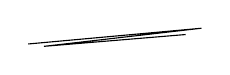
\begin{tikzpicture}\draw (0,0)--(2.2,.2)--(.2,-.03)--(2,.12);\end{tikzpicture}}

Comment opère $\sigma$ dans les quotients ?
\margin{\diagram{\begin{tikzcd}[row sep=large]
\sigma\quad P^1\arrow[d,"f"]\\
\sigma'\quad P^1\arrow[d,"g"]\\
\sigma''\quad P^1
\end{tikzcd}}}
On voit que $\sigma'(\infty)=0$, $\sigma'(0)=\infty$, $\sigma'(1)=1$, d'où mêmes formules pour $\sigma''$, d'où
\[
\deleted{\sigma'(t)=1/t}
\]
\deleted{et d'autre part}
\[
(11)\qquad\sigma'(t)=\sigma''(t)=1/t
\]
et il \unsure{serait} facile de \unsure{prouver} ces équations \unsure{pour $\sigma$ dans ce dernier cas} (p.ex.).
\figure{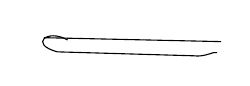
\begin{tikzpicture}\draw (0,.1) .. controls (-.25,.25) and (-.5,.05) .. (-.13,-.05)--(1.6,-.1) .. controls (1.75,-.12) and (1.85,-.04) .. (1.9,-.06);\draw (-.3,.13)--(1.95,.08);\end{tikzpicture}}
\mspage{39}

\scanpage{41}
\begin{center}- 18 -\end{center}
\hfill n$^\circ$ 276

un module filtré $(E,E_n)$ sur un anneau filtré $(A,A_n)$, et soit $\hat E$ le complété du groupe abélien $E$ muni de la topologie associée à la filtration donnée $\hat E$ est donc un groupe topologique abélien, d'ailleurs métrisable puisque la topologie de $E$ est définie par un écart. Comme les sous-groupes $E_n$ forment un système fondamental de voisinages de 0 dans $E$, \uline{les sous-groupes} $\hat E_n$ \uline{forment de même un système fondamental de voisinages de} 0 \uline{dans le groupe} $\hat E$ et si $F$ est un sous-groupe de $E$, muni de la topologie induite, le complété de $E/F$ n'est autre que $\hat E/\hat F$. Prenant $F=E_n$ et observant que, $E_n$ étant ouvert, le quotient $E/E_n$ est discret et donc complet, on voit que \uline{les homomorphismes canoniques}
\[
E/E_n\longrightarrow\hat E/\hat E_n
\]
\uline{sont bijectifs}. On notera d'autre part que, $E_n$ étant fermé, on a, lorsque $E$ est séparé (i.e. se plonge biunivoquement dans $\hat E$), la relation.
\[
E_n=E\cap\hat E_n.
\]
Considérons plus particulièrement l'anneau filtré $(A,A_n)$ lui-même ; Alors $\hat A$ est un \uline{anneau topologique} (\uline{Top.Gén.} Chap.III, \S\ 5, n$^\circ$4) et les relations $A_pA_q\subset A_{p+q}$ conduisent aux relations $\hat A_p\hat A_q\subset\hat A_{p+q}$ ; les sous-groupes $\hat A_p$ définissent donc une filtration de l'anneau $\hat A$, et comme ils forment un système fondamental de 0 on voit que la topologie de $A$ est précisément définie par cette filtration. Autrement dit, \uline{le complété de l'anneau filtré} $(A,A_n)$ \uline{est l'anneau filtré} $(\hat A,\hat A_n)$. Comme de plus $\hat A/\hat A_n$ s'identifie canoniquement à $A/A_n$ il est clair que \uline{les anneaux gradués associés} $G(A)$ \uline{et} $G(\hat A)$ \uline{sont canoniquement isomorphes}.

Revenant à un module filtré $(E,E_n)$ sur l'anneau filtré $(A,A_n)$, la loi de composition $A\times E\longrightarrow E$ se prolonge en une loi de composition $\hat A\times\hat E\longrightarrow\hat E$ on vérifie immédiatement qu'elle fait de $\hat E$ un $\hat A$-module ; comme de plus les
\mspage{40}

\scanpage{42}
Soit $S$ un schéma de base, et soit $X$ un schéma de Br. Severi sur $S$ muni d'une \uline{\unsure{trisection}} non ramifiée $X'$, i.e. un ss-schéma \inserted{fermé} de $X$ qui est non ramifié sur $X$, d'ordre 3 sur $X$. Un tel truc peut être considéré comme un objet à \unsure{schém.} structural $\mathfrak S_3$, opérant sur $P^1_S$ comme il a été dit. La classification de tels objets est donc la même que la classification dans un $H^1(S,\mathfrak S_3)$ des revêtts \inserted{gal.} \uline{non ramifiés} de groupe $\mathfrak S_3$ de $S$. De plus, $\sigma$ définit dans $X$ un $S$-automorphisme \inserted{involutif} \unsure{intr.} $\unsure{\sigma_S|\sigma}$ qui transforme $X'$ en un $X''$, dit \uline{associé} à $X'$. Évidt, si on partait de $(X,X'')$, on aurait le même $\sigma$, et \unsure{on restitue} $X'$ [à préciser\ldots]. De plus, on obtient [par descente\ldots] une \uline{bisection}, non ramifiée \deleted{\unsure{[en ses points}} en les pts de $S$ de car. $\ne2,3$]..... On peut passer au quotient, \deleted{\unsure{f}} par $\mathfrak S_3$, \deleted{\unsure{puis}} on trouve \unsure{par} :
\[
P^1_S\xrightarrow{p}P^1_S\quad\text{(comp. car }\mathfrak S_3\text{ opère}
\]
\mspage{41}

\scanpage{43}
\begin{center}- 17 -\end{center}
\hfill n$^\circ$ 276
\[
w:\widehat{E/F}\longrightarrow\widehat{\hat E/\hat F}
\]
Il est clair que $w\circ v$ n'est autre que l'application canonique de $\hat E/\hat F$ dans son complété ; si de plus l'on prolonge $v$ en une représentation
\[
\hat v:\widehat{\hat E/\hat F}\longrightarrow\widehat{E/F}
\]
alors $\hat v\circ w$ est l'identité, puisque c'est déjà l'identité sur $E/F$.

\uline{Si} $\hat E/\hat F$ \uline{est complet}, il résulte de ce qui précède que $v$ et $w$ sont des représentations inverses l'une de l'autre, autrement dit que $v$ est un isomorphisme du groupe topologique $\hat E/\hat F$ sur le groupe topologique $\widehat{E/F}$. D'après la prop.4, de \uline{Top. Gén.} Chap.IX, \S3, ce sera toujours le cas si le groupe $E$ est \uline{métrisable} puisqu'alors $\hat F$ est un sous-groupe fermé du groupe métrisable et complet $\hat E$. Il en sera de même plus généralement si la topologie de $E$ peut être définie à l'aide d'un écart.

On déduit de là le résultat suivant :

\uline{Lemme} 1 - \uline{Soient} $E,F,G$ \uline{trois groupes topologiques abéliens métrisables}, $u:E\longrightarrow F$ \uline{et} $v:F\longrightarrow G$ \uline{deux homomorphismes topologiques telle que la suite de groupes abéliens} $E\xrightarrow{u}F\xrightarrow{v}G$ \uline{soit} \uuline{exacte}. \uline{Alors} $\hat u:\hat E\to\hat F$ \uline{et} $\hat v:\hat F\longrightarrow\hat G$ \uline{sont des homomorphismes topologiques et la suite} $\hat E\xrightarrow{\hat u}\hat F\xrightarrow{\hat v}\hat G$ \uline{est exacte}.
\margin{\figure{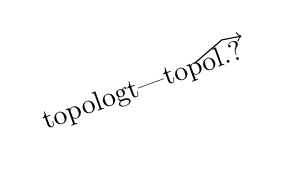
\begin{tikzpicture}\node[rotate=20] at (0,0) {\unsure{topologt|topol.?}};\draw[->] (.65,.3)--(1,.6)--(1.25,.65);\end{tikzpicture}}}

On a vu en effet, que le lemme 1 est vrai lorsque $u$ est injectif et $v$ surjectif. Or dans le cas général, la suite exacte donnée se décompose en suites exactes partielles,
\diagram{\begin{tikzcd}[column sep=small]N\arrow[r]&E\arrow[r]&I\end{tikzcd}\ ;\quad\begin{tikzcd}[column sep=small]I\arrow[r]&F\arrow[r]&J\end{tikzcd}\ ;\quad\begin{tikzcd}[column sep=small]J\arrow[r]&G\arrow[r]&K\end{tikzcd}}
qui rentrent dans ce cas particulier, et auxquelles le lemme 1 est donc applicable ; d'où évidemment le résultat cherché puisque le composé de deux homomorphismes est un homomorphisme.

Ces préliminaires sur les groupes topologiques étant rappelés, considérons
\mspage{42}

\scanpage{44}
trivialement sur le deuxième facteur) un morphisme naturel [aux \uuline{\unsure{pts} de car. $\ne2,3$}]
\[
X\xrightarrow{j}P^1_S
\]
qui est ramifié sur les sections $0$ \deleted{$\unsure{\infty}$}, $\infty$, $1$ \deleted{\unsure{et}} exclusivement : l'image inverse de $\infty$ est $X'$, celle de $0$ est $X''$, celle de $1$ \deleted{\unsure{est}} $X_1$.
\margin{(\uline{\unsure{aux dits pts}})}
\figure{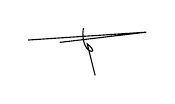
\begin{tikzpicture}\draw (0,0)--(1.5,.1)--(.4,-.03);\draw (.7,.15) .. controls (.65,-.2) and (.95,-.2) .. (.75,-.05)--(.85,-.45);\end{tikzpicture}}

Supposons maintenant que de plus, on se soit donné une section $s$ de $X\deleted{\unsure{_S}}$ sur $S$, ne rencontrant pas $X'$ (i.e. une section de $X-X'$ sur $S$). Son image par $j$ est alors une section de $P^1_S-(\infty)$, i.e. une section de $\underline O_S$, appelée \uline{l'invariant} de $(X,X',\deleted{\unsure{j}}s)$, soit \deleted{\unsure{j}} $\unsure{i|j}$.

Supposons que l'invariant $\unsure{j|i}$ ne prenne nulle part les valeurs $0,1$ i.e. soit inversible, ainsi que $\unsure{j|i}-1$. Alors son image inverse dans $P^1_S$ \deleted{\unsure{x}} de $p:S\to P^1_S$ définit un \deleted{section} \inserted{revêtement} \uline{galoisien} \uline{de} $S$, \uline{non ramifié}, \uline{de groupe} $\mathfrak S_3$, \deleted{\unsure{et}} \uline{et c'est celui qui définit} $X$. [\unsure{À déduire des formalismes|À déduire les formules}
\mspage{43}

\scanpage{45}
\begin{center}- 16 -\end{center}
\hfill n$^\circ$ 276

En effet, utilisons la filtration de $U(g)$ définie au n$^\circ$2, Exemple 3 ; elle est discrète : $U(g)$ est donc un anneau filtré séparé et complet ; or l'anneau gradué associé est un quotient d'un anneau de polynômes sur $K$, donc est noethérien ; d'où le corollaire.

7. - \uline{Complété d'un module filtré}.

Soit $E$ un groupe topologique abélien. Rappelons (Top. Gén.\unsure{.;}) que le complété $\hat E$ de l'espace uniforme $E$ est canoniquement muni d'une structure de groupe abélien, et que l'application canonique de $E$ dans $\hat E$ est une \uline{représentation} du groupe topologique $E$ dans le groupe topologique $\hat E$, dont le noyau est l'adhérence de 0 dans $E$.

Etant donné une \uline{représentation} $u$ de $E$ dans un groupe topologique abélien $E'$, l'application $u$ est uniformément continue, et par suite se prolonge en une application $\hat u:\hat E\longrightarrow\hat E'$ ; celle-ci est encore une \uline{représentation}

En particulier, soit $F$ un sous-groupe de $E$; l'application identique $j:F\longrightarrow E$ se prolonge en une représentation $\hat j$ du complété $\hat F$ dans le complété $\hat E$, laquelle est en fait un isomorphisme topologique de $\hat F$ sur un sous-groupe fermé de $\hat E$, à savoir l'adhérence de l'image de $F$ par l'application canonique de $E$ dans $\hat E$ ; nous identifierons toujours $\hat F$ à son image dans $\hat E$.

Considérons de plus le groupe topologique quotient $H=E/F$ ; la représentation canonique $E\xrightarrow{u}H$ se prolonge en une représentation $\hat E\xrightarrow{\hat u}H$, et comme $u$ applique $F$ sur $e$ il est clair que $\hat u$ applique $\hat F$ sur $e$ ; donc $\hat u$ définit par passage au quotient une représentation canonique
\[
v:\hat E/\hat F\longrightarrow\widehat{E/F}.
\]
On a d'autre part, à partir des représentations canoniques $E\to\hat E$ et $F\longrightarrow\hat F$, une représentation $E/F\to\hat E/\hat F$ et par suite une représentation
\mspage{44}

\scanpage{46}
catégoriques généraux \ldots\ ].

Donc en ce cas, l'invariant suffit à réconstituer \deleted{\unsure{toute}} la situation $(X,X',s)$.

Dans le cas où $X$ est normal, intègre, et où \uline{$i$ n'est pas identiquement égal à $0$ ou $1$}, \unsure{comme on connaît} le \unsure{revêt} non ramifié de $X$ sur l'ouvert $U$ où $i$ et $i-1$ inversibles $[S_{i(i-1)}]$, on le normalise partout, d'où reconstitution de $(X,X')$; d'autre part, on connaît $s$ sur $U$, donc ($X$ normal) partout.

Donc ici encore, \uline{$i$ permet de tt reconstituer}. Ici cependant, \unsure{se pose la} question : quels $i$ conviennent ??

Il faut exprimer (i) qu'une certaine extension de corps -- de degré $3$ -- du corps des fonctions de $X$ est non ramifié sur $X$ (ii) Qu'une certaine application rationnelle de $X$ qui s'en déduit est partout définie \ldots
\mspage{45}

\scanpage{47}
\begin{center}- 15 -\end{center}
\hfill n$^\circ$ 276

linéaire des $\alpha_{rs}X^r$ si $r\leq n$, et des $\alpha_{ns}X^r$ si $r>n$, d'où évidemment notre assertion.

(La démonstration précédente ne semble pas présenter d'avantage très décisif par rapport à la démonstration classique \ldots)

\uline{Corollaire 1} -- \uline{Soit} $K$ \uline{un corps} ; \uline{l'anneau de polynômes} $K[X_1,\ldots,X_r]$ \uline{est noethérien}.

On raisonne par récurrence sur $r$.

\margin{?}
\uline{Corollaire} 2 -- \uline{Soit} $A$ \figure{\begin{tikzpicture}[baseline=(n.base)]\node[draw,ellipse,inner sep=2pt] (n) {\uline{un anneau commutatif noethérien}};\end{tikzpicture}}. \uline{L'anneau de séries formelles} $A[[X]]$ \uline{est noethérien}.

Filtrons $A[[X]]$ par les puissances de l'idéal $(X)$ ; on obtient un anneau séparé et complet (Corollaire de la Proposition 5) ; or l'anneau gradué associé, isomorphe à $A[X]$, est noethérien ; donc $A[[X]]$ est noethérien en vertu du corollaire 2 de la proposition 7.

\uline{Corollaire} 3 -- \uline{Soit} $K$ \figure{\begin{tikzpicture}[baseline=(n.base)]\node[draw,ellipse,inner sep=3pt] (n) {\uline{un corps}};\end{tikzpicture}} ; \uline{l'anneau de séries formelles} $K[[X_1,\ldots,X_r]]$ \uline{est noethérien}.
\margin{\figure{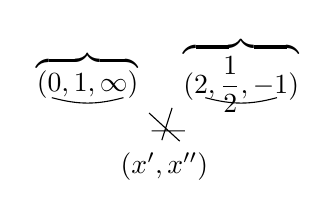
\begin{tikzpicture}[scale=.65]\node at (-1.5,1.1) {$\overbrace{(0,1,\infty)}$};\node at (1.5,1.1) {$\overbrace{(2,\frac12,-1)}$};\node at (0,-.7) {$(x',x'')$};\draw (-.25,0)--(.4,0) (-.05,-.18)--(.15,.45) (-.3,.35)--(.3,-.2);\draw (-2.2,.65) to[bend right=15] (-.8,.65);\draw (.8,.65) to[bend right=15] (2.2,.65);\end{tikzpicture}}}

Cela résulte du corollaire précédent par récurrence sur $r$.

Le corollaire 2 résulte aussi du suivant :

\uline{Corollaire} 4 -- \uline{Soient} $A$ \uline{un anneau commutatif et} $\mathrm m$ \uline{un idéal de} $A$. \uline{Supposons} $A/\mathrm m$ \uline{noethérien}, $\mathrm m$ \uline{à engendrement fini}, \uline{et} $A$ \uline{séparé et complet pour la topologie} $\mathrm m$-\uline{adique}. \uline{Alors} $A$ \uline{est noethérien}.

En effet, si $\mathrm m$ est engendré par des éléments $x_i$ en nombre fini dont nous noterons $\bar x_i\in G_1(A)$ les formes initiales, il est clair que tout élément de $G(A)$ est un polynôme en les $\bar x_i$, à coefficients dans l'anneau $G_0(A)=A/\mathrm m$ ; $G(A)$ est donc noethérien, d'où le résultat.

\uline{Corollaire} 5 -- \uline{Soit} $g$ \uline{une algèbre de Lie sur un anneau commutatif noethérien} $K$. \uline{L'algèbre enveloppante de} $g$ \uline{est un anneau noethérien (à gauche et à droite)}
\mspage{46}

\scanpage{48}
\deleted{\unsure{Supposons} $i$ \unsure{est égal à} $\unsure{0}$}

En tous cas, si $i=0$, la situation est décrite par le fait que l'on a fait une réduction du groupe structural de $\mathfrak S_3$ à $\mathbb Z/2$ \inserted{[$X''$ \inserted{\unsure{donc $X'$}} a une section !]}, et que \unsure{Tout} est déterminé par la donnée d'un élément de $H^1(S,\mathbb Z/2)$. \deleted{\unsure{Supposons}} \inserted{Et} si $i=1$, alors la situation est décrite en disant que l'on a une réduction du groupe structural à $\mathbb Z/3\subset\mathfrak S_3$ [\unsure{grâce} à une section de \inserted{la bisection} $X_1$] et la situation est décrite par la donnée d'un élément de $H^1(S,\mathbb Z/3)$.

\figure{\begin{tikzpicture}\draw (0,0)--(3,0);\end{tikzpicture}}

\deleted{\unsure{Donc}} En tous les cas encore, si $i$ est inversible, alors faisons opérer $\mathfrak S_3$ sur $P^1_S/(\mathbb Z/3)$ par passage au quotient, on trouve dans \deleted{\unsure{ce dernier}} \inserted{\unsure{ce fibré conique}} \deleted{\unsure{deux}} \uline{trois sections} distinctes, \inserted{(provenant de $X',\unsure{X''|X'''}$ et $s$)} que l'on peut choisir comme $\infty,0,1$, d'où une identification de ce dernier à $P^1_S$, et $X\longrightarrow P^1_S$ se factorise par
\diagram{\begin{tikzcd}[column sep=large,row sep=small]
X\arrow[r]&P^1_S\arrow[r]&P^1_S\\
&\infty,0,1\arrow[r]&\infty,0,i\\
&t\arrow[r,no head]&it^2
\end{tikzcd}}
; la bisection naturelle en question s'identifie alors à $\sqrt i$ ;
\mspage{47}

\scanpage{49}
\mspage{48}
\begin{center}- 13 -\end{center}
\hfill n$^\circ$;276

de la proposition précédente il suffit pour cela de faire voir que l'homomorphisme associé $G(u)$ est surjectif, autrement dit que pour tout $x\in E_n$ il existe des $a_i\in A_{n-p_i}$ tels que l'on ait $x\equiv a_ix_i\pmod{E_{n+1}}$ ; mais cela signifie précisément que les $\tilde x_i$ engendrent le $G(A)$-module $G(E)$ : en effet, si $\tilde x\in G_n(E)$, on peut trouver des $\tilde a_i\in G(A)$ tels que $\tilde x=\sum\tilde a_i\tilde x_i$, et cette relation subsiste si l'on remplace $\tilde a_i$ par sa composante de degré $n-p_i$.

\uline{Corollaire} 1 -- \uline{Soit} $E$ \uline{un module filtré séparé sur un anneau filtré complet} $A$; \uline{Si} $G(E)$ \uline{est} \inserted{un} $G(A)$-\uline{module de type fini} (resp. \uline{noethérien}) \uline{alors} $E$ \uline{est un} $A$-\uline{module de type fini} (resp. \uline{noethérien}).

Soit en effet $F$ un sous-module de $E$, et munissons le de la filtration induite ; $G(F)$ est alors un sous-module homogène du $G(A)$-module gradué $G(E)$ ; si $G(F)$ est de type fini, on peut l'engendrer à l'aide d'éléments homogènes en nombre fini -- il suffit pour le voir de prendre les composantes homogènes d'un système fini de générateurs de $G(F)$ ; en considérant des;éléments de $F$ dont ces générateurs sont les formes initiales on voit, à l'aide de la Proposition 7, que $F$ est lui-même un module de type fini, d'où immédiatement le corollaire.

\uline{Corollaire} 2 -- \uline{Soit} $(A,A_n)$ \uline{un anneau filtré séparé et complet} ; \uline{si} $G(A)$ \uline{est un anneau noethérien à gauche}, $A$ \uline{est noethérien à gauche}.

Il suffit d'appliquer le corollaire précédent à $E=A$.

\uline{Corollaire} 3 -- \uline{Soient} $A$ \uline{un anneau}, $\mathrm m$ \uline{un idéal bilatère de} $A$, \uline{et} $E$ \uline{un} $A$-\uline{module}. \uline{Supposons} $A$ \uline{complet et} $E$ \uline{séparé pour la topologie} $\mathrm m$-\uline{adique}. \uline{Si des éléments} $x_i\in E$, \uline{en nombre fini, engendrent le} $A$-\uline{module} $E/\mathrm m.E$, \uline{ils engendrent} $E$.

D'après la Proposition 7, il suffit de montrer que les éléments $\tilde x_i\in E/\mathrm m E=G_0(E)$ engendrent le $G(A)$-module $G(E)$, autrement dit que, pour

\scanpage{50}
\deleted{\unsure{Autre façon}}

Ceci ne nous a pas donné de façon très explicite de classifier les ``courbes \inserted{\unsure{simples}} de genre $0$'' sur $S$, munies d'une section et d'une trisection non ramifiée, disjointes
\margin{\figure{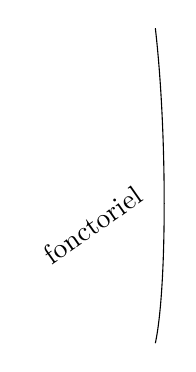
\begin{tikzpicture}[x=1cm,y=1cm]\node[rotate=35] at (-.8,0) {fonctoriel};\draw (0,2.5) .. controls (0.15,1.2) and (.15,-.8) .. (0,-1.5);\end{tikzpicture}}}
[\deleted{$\unsure{X}$} $=$ \unsure{revêtement} $\unsure{\mathfrak S_3}$ \unsure{non} ramifié \inserted{$S'$} de groupe $\mathfrak S_3$ de $S$, avec une section \deleted{de} de
\[
\deleted{\unsure{X\simeq P^1_S\times_{(S,\mathfrak S_3)}}}\quad S'\times_{(S,\mathfrak S_3)}\unsure{\mathbf P|P}^1_S
\]
\inserted{$t$ disjoint de $0,1,\infty$,} invariant par le groupe $\mathfrak S_3$, i.e. \deleted{une section}
\[
t\in\Gamma(S',\underline O_{S'}),
\]
inversible et telle que $t-1$ soit inversible, et satisfaisant à
\[
\sigma.t=\deleted{\unsure{\varphi}}\unsure{\bar\sigma}(t)\qquad\sigma\in\mathfrak S_3
\]
i.e.
\[
\begin{cases}\lambda t=\dfrac1t\\\mu t=1-t\end{cases}
\]
\margin{\diagram{\begin{tikzcd}X\arrow[d]&P^1_{S'}\arrow[l]\arrow[d]\\S&S'\arrow[l,"\mathfrak S_3"']\end{tikzcd}}}
\figure{\begin{tikzpicture}\draw (0,1.2) to[bend right=8] (0,.2)--(.25,0);\end{tikzpicture}}

\margin{\uuline{non} \uline{fonctoriel}}
\uline{Exemple} $S=\operatorname{Spec}(O)$, $O$ anneau local \uline{complet} à corps résiduel $\mathrm{alg.}^{\mathrm t}$ clos \deleted{\unsure{(car. $\ne2,3$)}} \inserted{(de car. $\ne2,3$)}.

Alors \deleted{$\unsure{X\simeq P^1_S}$} $\pi_1(S)=0$, donc la situation équivaut, \inserted{[\unsure{Donn. non canoniq.|Donn. non canonique} \unsure{par} \unsure{quoi}]} à la donnée d'un $t\in O^*$ tel que \deleted{$\unsure{t(t-1)\in\mathbb Z}$} $t(t-1)\in O^*$, étant entendu que $t,t'$ donnent des \unsure{représ.} isomorphes \deleted{\unsure{si et}} s. s. s. $t'$ est de la forme \inserted{$\bar\sigma(t)\quad\sigma\in\mathfrak S_3$.}
\mspage{49}
